%% abtex2-modelo-trabalho-academico.tex, v-1.4 laurocesar
%% Copyright 2012-2013 by abnTeX2 group at http://abntex2.googlecode.com/ 
%%
%% This work may be distributed and/or modified under the
%% conditions of the LaTeX Project Public License, either version 1.3
%% of this license or (at your option) any later version.
%% The latest version of this license is in
%%   http://www.latex-project.org/lppl.txt
%% and version 1.3 or later is part of all distributions of LaTeX
%% version 2005/12/01 or later.
%%
%% This work has the LPPL maintenance status `maintained'.
%% 
%% The Current Maintainer of this work is the abnTeX2 team, led
%% by Lauro César Araujo. Further information are available on 
%% http://abntex2.googlecode.com/
%%
%% This work consists of the files abntex2-modelo-trabalho-academico.tex,
%% abntex2-modelo-include-comandos and abntex2-modelo-references.bib
%%

% ------------------------------------------------------------------------
% ------------------------------------------------------------------------
% abnTeX2: Modelo de Trabalho Acadêmico (tese de doutorado, dissertação de
% mestrado e trabalhos monográficos em geral) em conformidade com 
% ABNT NBR 14724:2011: Informação e documentação - Trabalhos acadêmicos -
% Apresentação
% ------------------------------------------------------------------------
% ------------------------------------------------------------------------


\documentclass[
	% -- opções da classe memoir --
	12pt,				% tamanho da fonte
	openright,			% capítulos começam em pág ímpar (insere página vazia caso preciso)
	oneside,			% para impressão em verso e anverso. Oposto a oneside
	a4paper,			% tamanho do papel. 
	% -- opções da classe abntex2 --
	%chapter=TITLE,		% títulos de capítulos convertidos em letras maiúsculas
	%section=TITLE,		% títulos de seções convertidos em letras maiúsculas
	%subsection=TITLE,	% títulos de subseções convertidos em letras maiúsculas
	%subsubsection=TITLE,% títulos de subsubseções convertidos em letras maiúsculas
	% -- opções do pacote babel --
	english,			% idioma adicional para hifenização
%	french,				% idioma adicional para hifenização
%	spanish,			% idioma adicional para hifenização
	brazil				% o último idioma é o principal do documento
	]{abntex2}

% ---
% PACOTES
% ---

% ---
% Pacotes fundamentais
%\usepackage{subfig}
\usepackage{amsmath}
\usepackage{tocloft}
\usepackage{cmap}				% Mapear caracteres especiais no PDF
\usepackage{lmodern}			% Usa a fonte Latin Modern			
%\usepackage{fourier}
%\usepackage[portuges,brazil]{babel}
\usepackage[T1]{fontenc}		% Seleção de códigos de fonte.
\usepackage[utf8]{inputenc}		% Determina a codificação utiizada (conversão automática dos acentos)
\usepackage{makeidx}            % Cria o indice
\usepackage{amssymb,amsfonts,amsmath,wasysym}
%\usepackage{hyperref}  			% Controla a formação do índice
%\usepackage{cleveref}
\usepackage{lastpage}			% Usado pela Ficha catalográfica
\usepackage{indentfirst}		% Indenta o primeiro parágrafo de cada seção.
\usepackage{nomencl} 			% Lista de simbolos
\usepackage{color}				% Controle das cores
\usepackage{graphicx}			% Inclusão de gráficos
\usepackage{microtype} 			% para melhorias de justificação
\usepackage{subfig}
\usepackage{float} % Colocar a figura no local certo
\usepackage{scalefnt} % Pacote da redimensionar a fonte de tabelas, figuras e equações.
\usepackage{placeins}
\allowdisplaybreaks
\usepackage{kantlipsum}
%\usepackage{showframe}
%\renewcommand{\rmdefault}{phv} % Arial
%\renewcommand{\sfdefault}{phv} % Arial
\usepackage{pdfpages}
\usepackage{titlesec}

%\titleformat{\section}{\normalfont\scshape}{\thesection}{1em}{}
%\titlespacing{\section}{0pt}{12pt}{6pt} 


\renewcommand{\figurename}{Figura-}
\usepackage[figurename=Figura]{caption}

% ---

\renewcommand{\chapnumfont}{\bfseries}

\renewcommand{\ABNTEXfontereduzida}{\mdseries\footnotesize}
%\renewcommand{\ABNTEXchapterfont}{\bfseries\sffamily}

%\renewcommand{\ABNTEXsubsectionfont}{\fontseries{n}\selectfont}
%\renewcommand{\ABNTEXsubsubsectionfont}{\fontseries{it}\selectfont}
%
%\renewcommand{\ABNTEXpartfontsize}{\normalsize}
\renewcommand{\ABNTEXchapterfontsize}{\bfseries \normalsize}%{\Large}
\renewcommand{\ABNTEXsectionfontsize}{\normalsize}%{\large}
%\renewcommand{\ABNTEXsubsectionfontsize}{\normalsize}
%\renewcommand{\ABNTEXsubsubsectionfontsize}{\normalsize}

%\renewcommand{\agradecimentosname}{\textbf{AGRADECIMENTOS}}
%\renewcommand{\resumoname}{\textbf{RESUMO}}
%\renewcommand{\contentsname}{\textbf{SUMÁRIO}}
%\renewcommand\contentsname{\textbf{SUMÁRIO}}
\addto{\captionsbrazil}{\renewcommand{\contentsname}{\textbf{SUMÁRIO}}}
%\addto{\captionsbrazil}{\renewcommand{\listfigurename}{\textbf{LISTA DE ILUSTRAÇÕES}}}
\addto{\captionsbrazil}{\renewcommand{\bibname}{\bfseries \textbf{REFERÊNCIAS}\selectfont}}
%\addto{\captionsbrazil}{\renewcommand{\appendixname}{\bfseries\MakeUppercase{APÊNDICES}}}

\renewcommand{\apendicesname}{\bfseries \selectfont  APÊNDICES}
\renewcommand{\apendicename}{\bfseries\selectfont APÊNDICE}
\renewcommand{\anexosname}{\bfseries ANEXOS}
%\chapterstyle{ell}
% ---
% Pacotes adicionais, usados apenas no âmbito do Modelo Canônico do abnteX2
% ---
\usepackage{lipsum}				% para geração de dummy text
% ---


% ---
% Pacotes de citações
% ---
\usepackage[brazilian,hyperpageref]{backref}	 % Paginas com as citações na bibl
\usepackage[alf]{abntex2cite}	% Citações padrão ABNT

% CONFIGURAÇÕES DE PACOTES
% --- 
% ---
% Configurações do pacote backref
% Usado sem a opção hyperpageref de backref
%\renewcommand{\backrefpagesname}{Citado na(s) página(s):~}
%\renewcommand{\backrefpagesname}{}
% Texto padrão antes do número das páginas
%\renewcommand{\backref}{}
% Define os textos da citação
%\renewcommand*{\backrefalt}[4]{
%	\ifcase #1 %
%		Nenhuma citação no texto.%
%	\or
%		Citado na página #2.%
%	\else
%		Citado #1 vezes nas páginas #2.%
%	\fi}%
% ---
\renewcommand*{\backrefalt}[4]{
	\ifcase #1 %
	
	\or
	
	\else

	\fi}%
% Informações de dados para CAPA e FOLHA DE ROSTO
% ---



\instituicao{%
  Universidade Federal do Pará -- UFPA
  \par
  Instituto de Geociências
  \par
  Programa de Pós-Graduação em Geofísica}
\titulo{APROXIMAÇÕES DE PADÉ PARA O CRS ZERO OFFSET}

\autor{Rodolfo André Cardoso Neves}
\local{Belém-Pará}
\data{2018}

\orientador{Prof. Dr. João Carlos Ribeiro Cruz}
\coorientador{}

%\tipotrabalho{Mestrado}
% O preambulo deve conter o tipo do trabalho, o objetivo, 
% o nome da instituição e a área de concentração 
\preambulo{Tese apresentada ao Programa de Pós-Graduação em Geofísica do Instituto de Geociências 
da Universidade Federal
do Pará, em cumprimento às exigências para obtenção do grau de Doutor em Geofísica.}
% ---



% ---
% Configurações de aparência do PDF final

% alterando o aspecto da cor azul
\definecolor{blue}{RGB}{41,5,195}
\definecolor{black2}{RGB}{39,64,139}
% informações do PDF
\hypersetup{
		backref=true,
		pagebackref=true,
		bookmarks=true,         		% show bookmarks bar?
		pdftitle={\imprimirtitulo}, 
		pdfauthor={\imprimirautor},
    	pdfsubject={\imprimirpreambulo},
		pdfkeywords={PALAVRAS}{CHAVES}{abnt}{abntex}{abntex2},
	    pdfproducer={LaTeX with abnTeX2}, 	% producer of the document
	    pdfcreator={\imprimirautor},
    	colorlinks=true,       		% false: boxed links; true: colored links
    	linkcolor=black,          	% color of internal links
    	citecolor=black,        		% color of links to bibliography
    	linkcolor=black,          	% color of internal links
    	citecolor=black,        		% color of links to bibliography
    	filecolor=black,      		% color of file links
		urlcolor=black,
		bookmarksdepth=4
}
% --- 

% --- 
% Espaçamentos entre linhas e parágrafos 
% --- 

% O tamanho do parágrafo é dado por:
\setlength{\parindent}{1.3cm}

% Controle do espaçamento entre um parágrafo e outro:
\setlength{\parskip}{0.2cm}  % tente também \onelineskip

% Controles do espaçamento entre linhas:
\OnehalfSpacing	% espaçamento um e meio (padrão); 
%\DoubleSpacing		% espaçamento duplo
%\SingleSpacing		% espaçamento simples	
% --- 
	

% ---
% compila o indice
% ---
\makeindex
% ---

% ---
% Compila a lista de abreviaturas e siglas
% ---
\makenomenclature
% ---

\usepackage{tensor}

\renewcommand{\sin}{\mathrm{sen}}
\newcommand{\disp}{\displaystyle}
\newcommand{\mbf}{\mathbf}

\hyphenation{geo-fí-si-co}
\hyphenation{MCSEM}



% Numeração por capítulo das figuras
%\counterwithin{figure}{chapter}
%\counterwithin{table}{chapter}
% ---
%\usepackage{subfigure}
\usepackage{setspace}
\usepackage{caption}
%\captionsetup{format=hang,labelsep=period,margin=10pt,font=small,justification=justified,labelfont=md}
\captionsetup{labelsep=period,font=small,justification=justified,labelfont=md,format=plain,labelsep=endash}





\renewcommand{\imprimircapa}{%
\begin{capa}%
	\begin{figure}[!t]
		\begin{center}
			
\includegraphics[scale=0.3]{Logo_UFPA2.pdf}
		\end{center} 
	\end{figure}
			\begin{center}
				{\ABNTEXchapterfont\bfseries{UNIVERSIDADE FEDERAL DO PARÁ \\ INSTITUTO DE GEOCIÊNCIAS \\ PROGRAMA DE PÓS-GRADUAÇÃO EM GEOFÍSICA} }
		\end{center}
%\vspace*{2cm}

\center

\vspace*{1cm}
{\ABNTEXchapterfont\bfseries\large\MakeUppercase{\imprimirautor}}\\
\vspace*{2cm}
{\ABNTEXchapterfont\bfseries\large\imprimirtitulo}\\
\vspace*{2cm}
%			\begin{center}
				{\ABNTEXchapterfont\bfseries\large{PROJETO DE TESE DE DOUTORADO}}
%			\end{center}
%{\ABNTEXchapterfont\large\imprimirautor}
\vspace*{\fill}\\
{\large\MakeUppercase{\imprimirlocal}}
\par
{\large\imprimirdata}
\vspace*{1cm}
\end{capa}
}


\makeatletter
\renewcommand{\folhaderostocontent}{
\begin{center}
	\vspace*{1cm}
	{\ABNTEXchapterfont\bfseries\large\MakeUppercase{\imprimirautor}}\\
	\vspace*{\fill}\vspace*{\fill}
	{\ABNTEXchapterfont\bfseries\large\imprimirtitulo}\\
	 \vspace{\baselineskip}
	{\ABNTEXchapterfont\bfseries\large{PROJETO DE TESE DE DOUTORADO}}
	\vspace{\baselineskip}
	\vspace{\baselineskip}
	\vspace*{\fill}
	\abntex@ifnotempty{\imprimirpreambulo}{%
%	\hspace{.5\textwidth}
	\hspace{5cm}
	\begin{minipage}{10cm}
	\SingleSpacing
	\imprimirpreambulo\\ \\
	{\imprimirorientadorRotulo~Prof. Dr. João Carlos Ribeiro Cruz}\\
	%{\imprimircoorientadorRotulo~}
	\end{minipage}%
	\vspace*{\fill}
	}%
	
%	{\imprimirorientadorRotulo~\imprimirorientador}

	\abntex@ifnotempty{\imprimircoorientador}{%
	{\large\imprimircoorientadorRotulo~\imprimircoorientador}%
	}%
	\vspace*{\fill}
%%	{\abntex@ifnotempty{\imprimirinstituicao}{\imprimirinstituicao\vspace*{\fill}}}
	{\large\imprimirlocal}
	\par
	{\large\imprimirdata}
	\vspace*{1cm}
\end{center}

}

\makeatother








% ----
% Início do documento
% ----
%\usepackage{nohyperref}
%\renewcommand{\ABNTEXsectionfont}{\fontseries{m}\selectfont}
\begin{document}

% ----------------------------------------------------------
% ELEMENTOS PRÉ-TEXTUAIS
% ----------------------------------------------------------
% \pretextual

% ---
% Capa %%%%TROCAR ARQUIVO COM MINHAS 
% ---
\imprimircapa
% ---

% ---
% Folha de rosto %%%%TROCAR ARQUIVO COM MINHAS INFORMAÇÕES
% (o * indica que haverá a ficha bibliográfica)
% ---
\imprimirfolhaderosto*
% ---

% ---
% Inserir a ficha bibliografica
% ---

% Isto é um exemplo de Ficha Catalográfica, ou ``Dados internacionais de
% catalogação-na-publicação''. Você pode utilizar este modelo como referência. 
% Porém, provavelmente a biblioteca da sua universidade lhe fornecerá um PDF
% com a ficha catalográfica definitiva após a defesa do trabalho. Quando estiver
% com o documento, salve-o como PDF no diretório do seu projeto e substitua todo
% o conteúdo de implementação deste arquivo pelo comando abaixo:
%


%  

%\begin{fichacatalografica}
%	\vspace*{\fill}					% Posição vertical
%	\hrule							% Linha horizontal
%	\begin{center}					% Minipage Centralizado
%	\begin{minipage}[c]{12.5cm}		% Largura
%	
%	\imprimirautor
%	
%	\hspace{0.5cm} \imprimirtitulo  / \imprimirautor. --
%	\imprimirlocal, \imprimirdata-
%	
%	\hspace{0.5cm} \pageref{LastPage} p. : il. (algumas color.) ; 30 cm.\\
%	
%	\hspace{0.5cm} \imprimirorientadorRotulo~\imprimirorientador\\
%	
%	\hspace{0.5cm}
%	\parbox[t]{\textwidth}{\imprimirtipotrabalho~--~\imprimirinstituicao,
%	\imprimirdata.}\\
%	
%	\hspace{0.5cm}
%		1. Geofísica Aplicada.
%		2. Métodos Eletromagnéticos.
%		3. MCSEM 1D
%		4. MATLAB
%		5. Interface Gráfica
%		I. SOUZA, Victor Cezar Tocantins de. Orient.
%		II. Universidade Federal do Pará.
%		III. Faculdade de Geofísica.
%		IV. Título\\ 			
%	
%	\hspace{8.75cm} CDU XX:XXX:XXX.X\\
%	
%	\end{minipage}
%	\end{center}
%	\hrule
%\end{fichacatalografica}
% ---

% ---
% Inserir errata
% ---
%\begin{errata}
%Elemento opcional da \citeonline[4.2.1.2]{NBR14724:2011}. Exemplo:
%
%\vspace{\onelineskip}
%
%FERRIGNO, C. R. A. \textbf{Tratamento de neoplasias ósseas apendiculares com
%reimplantação de enxerto ósseo autólogo autoclavado associado ao plasma
%rico em plaquetas}: estudo crítico na cirurgia de preservação de membro em
%cães. 2011. 128 f. Tese (Livre-Docência) - Faculdade de Medicina Veterinária e
%Zootecnia, Universidade de São Paulo, São Paulo, 2011.
%
%\begin{table}[htb]
%\center
%\footnotesize
%\begin{tabular}{|p{1.4cm}|p{1cm}|p{3cm}|p{3cm}|}
%  \hline
%   \textbf{Folha} & \textbf{Linha}  & \textbf{Onde se lê}  & \textbf{Leia-se}  \\
%    \hline
%    1 & 10 & auto-conclavo & autoconclavo\\
%   \hline
%\end{tabular}
%\end{table}
%
%\end{errata}
% ---

% ---
% Inserir folha de aprovação
% ---

% Isto é um exemplo de Folha de aprovação, elemento obrigatório da NBR
% 14724/2011 (seção 4.2.1.3). Você pode utilizar este modelo até a aprovação
% do trabalho. Após isso, substitua todo o conteúdo deste arquivo por uma
% imagem da página assinada pela banca com o comando abaixo:
%

%\includepdf{Folha.pdf}
%
\setlength{\ABNTEXsignwidth}{11cm}
%\begin{folhadeaprovacao}
%\begin{center}
% {\ABNTEXchapterfont\bfseries\large\MakeUppercase{\imprimirautor}}
% \vspace*{\fill}\vspace*{\fill}
% \begin{center}
% \ABNTEXchapterfont\bfseries\large\imprimirtitulo
% \end{center}
% \vspace*{\fill}
% \hspace{.45\textwidth}
% \begin{minipage}{.5\textwidth}
% \imprimirpreambulo
% \end{minipage}%
% \vspace*{\fill}
% \end{center}
% Data de Aprova\c{c}\~ao:  03/07/2017 \\ \\ \\ 
% Banca Examinadora:
% \begin{center}
% \assinatura{Prof. Dr. João Carlos Ribeiro Cruz - Orientador \\ Universidade Federal do Par\'a -- UFPA}
% \assinatura{Prof. Dr. Paulo Eduardo Miranda Cunha - Membro  \\ Petrobrás}
% \assinatura{Prof. Dr. Rubenvaldo Pereira - Membro \\ Universidade Federal do Par\'a -- UFPA}
% \end{center}
%Suplentes:
%\begin{center}
%\assinatura{Professor Pedro Andres Chira Oliva \\ Doutor em geof\'sica \\ Universidade Federal do Par\'a -- UFPA}
%\assinatura{Professor Manuel de Jesus Costa\\ Doutor em geofísia \\ Universidade Federal do Par\'a -- UFPA}
%\end{center}
%\begin{center}
%\vspace*{0.5cm}
%{\large\imprimirlocal}
%\par
%{\large\imprimirdata}
%\vspace*{1cm}
%\end{center}
%\includepdf{Folha.pdf}
%\end{folhadeaprovacao}

% Dedicatória
% ---
\begin{dedicatoria}
   \vspace*{\fill}
   \vspace*{13cm}
   \centering
   \noindent
   \begin{flushright} Dedico este trabalho \`a minha fam\'ilia.
   \end{flushright}
     \vspace*{\fill}
\end{dedicatoria}
% ---


% ---
% Agradecimentos
% ---
\begin{agradecimentos}[\fontsize{12pt}{\baselineskip}\textbf{AGRADECIMENTOS}]
\vspace*{1.5cm}

Ao Prof. Dr. João Carlos pela orientação desta tese, e pela proposta do tema. Além
do suporte e paciência em responder as minhas dúvidas, e das sugestões inteligentes na solução de problemas
que foram aparecendo no caminho.

Agradeço ao professor Sergey Fomel, que apesar de não conhecer pessoalmente, produziu trabalhos
que inspiraram o tema, e disponibilizou gratuitamente
vários
dos programas aqui utilizados.

Agradeço à minha mãe Regina de Nazaré,
à minha irmã Rebeca Cristina, às minhas sobrinhas Ágatha e Anadora, e ao meu pai Ricardo Neves, por todo apoio e dedicação
durante a árdua caminhada para a realização deste sonho!

E agradeço à amizade de amigos que conquistei durante o curso de Geofísica, e que de forma direta ou indireta
me ajudaram na realização do trabalho:
Leonardo Reis, Hugo Souza, Diogo Rezende, Antônio Rizimar e Raphael Di Carlo.

\end{agradecimentos}
% ---

% ---
% Epígrafe
% ---
\begin{epigrafe}
    \vspace*{\fill}
	\begin{flushright}
		\textit{``Todas as coisas excelentes são tão difíceis quanto raras''. \\
		(Baruch Spinoza)}
	\end{flushright}
\end{epigrafe}
% ---

% ---
% RESUMOS
% ---

% resumo em português
\begin{resumo}[\fontsize{12pt}{\baselineskip}\textbf{RESUMO}]
\OnehalfSpacing	% espaçamento um e meio (padrão); 
O cálculo das derivadas da superfície Crs-Padé em relação aos parâmetros não é simples de ser feito,
sugiro a realização da inversão dos parâmetros do CRS através da otimização global para a aproximação de Padé.
 \vspace{\onelineskip} 
 \noindent
 \par Palavras-chave: Aproximantes de Padé. Aproximações não hiperbólicas do tempo de trânsito. Aproximações de Padé
 para a configuração ponto médio comum e configuração superfície de reflexão comum. 
\end{resumo}

% resumo em inglês
\begin{resumo}[\fontsize{12pt}{\baselineskip}\textbf{ABSTRACT}]
\OnehalfSpacing	% espaçamento um e meio (padrão); 
O cálculo das derivadas da superfície Crs-Padé em relação aos parâmetros não é simples de ser feito,
sugiro a realização da inversão dos parâmetros do CRS através da otimização global para a aproximação de Padé.
\vspace{\onelineskip} 
\noindent 
\par Keywords: Padé approximants. Non-hyperbolic traveltime aproximation. Padé aproximation CMP gather.
Padé aproximation CRS gather.
\end{resumo}

% ---
% inserir lista de ilustrações
% ---
\renewcommand{\listfigurename}{\fontsize{12pt}{\baselineskip}\textbf{LISTA DE ILUSTRAÇÕES}}
\pdfbookmark[0]{\listfigurename}{lof}
\listoffigures*

\cleardoublepage

% ---
% inserir lista de tabelas
% ---
%\pdfbookmark[0]{\listtablename}{lot}
%\listoftables*
%\cleardoublepage
% ---

% ---
% inserir lista de abreviaturas e siglas
% A lista de Abreviaturas e Siglas pode ser facilmente montada com o pacote 
% nomencl. Abaixo segue um exemplo.
% ---
%\nomenclature{Fig.}{Figura}
%\nomenclature{$A_i$}{Area of the $i^{th}$ component} 
%\nomenclature{456}{Isto é um número}
%\nomenclature{123}{Isto é outro número}
%\nomenclature{a}{primeira letra do alfabeto}
%\nomenclature{lauro}{este é meu nome} 
%
%\renewcommand{\nomname}{Lista de abreviaturas e siglas}
%\pdfbookmark[0]{\nomname}{las}
%\printnomenclature
%\cleardoublepage
% ---

% ---
% inserir lista de símbolos
% ---
% O abnTeX2 não provê mecanismo para lista de símbolos.
% ---

% ---
% inserir o sumario
% ---
%\renewcommand{\tocheadstart}{\ABNTEXchapterfont}
\pdfbookmark[0]{\contentsname}{toc}
%\settocdepth{chapter}


\tableofcontents*
%%%%%%%Colocar minhas informações
%\includepdf{SUMARIO.pdf}

\cleardoublepage
% ---



% ----------------------------------------------------------
% ELEMENTOS TEXTUAIS
% ----------------------------------------------------------
% É possível usar \textual ou \mainmatter, que é a macro padrão do memoir.  
\mainmatter

 \chapter{INTRODUÇÃO}
\label{intro}

Os eventos de difração trazem informações sobre as pequenas heterogeneidades em subsuperfície. Como falhas, fraturas
canais e flancos de domo de sal \cite{sep_dif}.
Portanto, apesar do processamento sísmico concentrar seus esforços no imageamento de ondas refletidas, o valor das
difrações não deve ser subestimado \cite{khaidukov}.

Em teoria, podemos separar difrações e reflexões no domínio dos dados: Ondas sísmicas refletidas e difratadas são
dois fenômenos físicos fundamentalmente distintos \cite{klen}. Partimos da hipótese de que, no volume dos dados
empilhados, correspondem a eventos fortemente coerentes com inclinações contínuas. Remover as reflexões, revelamos
as difrações.


Partindo da seção empilhada, nós propomos a identificação e remoção dos eventos de reflexão 
através do filtro de destruição de ondas planas 
\cite{claerbout}: O método de destruição de ondas planas estima a continuidade das inclinações 
locais dos eventos sísmicos dominantes
formando uma predição de cada dado no traço em relação aos traços na vizinhança com a otimização a partir de
filtros não estacionários compactos que seguem que seguem a energia sísmica ao longo das inclinações estimadas
\cite{sep_dif}.

Após a remoção das reflexões da seção empilhada, migramos a seção,
contendo apenas eventos de difração, múltiplas vezes. Para isto utilizamos
diferentes velocidades de migração em um processo chamado de \textit{velocity continuation}, a partir de um algoritmo baseado
na FFT \cite{sep_dif}.

Montamos os \textit{focusing image gathers} (FIG) calculando para cada ponto no domínio 
da imagem a sua \textit{variação máxima local},
para cada uma das imagens migradas produzidas no passo anterior a partir de uma velocidade de migração distinta. 
Para pontos no domínio da imagem que sejam pontos de foco (difrações), o valor da \textit{variação máxima local} é máximo. 
Assim o FIG é um painel que mostra os maiores valores de \textit{variação máxima local} 
para as velocidade de migração otimizadas (análise de velocidade de migração).

Obtemos a curva de tempo de trânsito do método do elemento de reflexão comum (ERC) para os pontos no domínio da imagem,
a partir de $R_N$ e $\beta_0$ obtidos do modelo de velocidades do passo anterior, otimizados a partir do algoritmo
very fast simulated aneeling (VFSA).
As coordenadas $m$ e $h$ e o tempo de trânsito da ERC são interpoladas a partir das aproximações
de tempo de trânsito SRC Padé \cite{neves} que tangencia a superfície de tempo de trânsito ERC.
A partir daí empilhamos sobre a curva de tempo de trânsito ERC no domínio dos dados e ressaltamos as difrações. %INTRODUÇÃO
 \include{sep_diff} %IMAGEAMENTO DE DIFRAÇÕES
%  \chapter{OBJETIVO}
\label{objetivo}


 %
 \chapter{OTIMIZAÇÃO GLOBAL COM SIMULATED ANNEALING}
\label{cap2}


O algoritmo Simulated Annealing é baseado na teoria física da formação de cristais
através do resfriamento lento (Annealing) destes cristais, a partir do seu ponto de fusão.
O objetivo é minimizar a função objeto $f(p)$ a patir de perturbações aleatórias do vetor de parâmetros $p$,
para uma nova posição $p'$. O valor $p'$ é avaliado a partir do seguinte critério de aceitação:

\begin{equation}
\label{eq:2.8}
 \Delta f=f(p')-f(p) < 0
\end{equation}

O algoritmo inicia através da escolha de um valor inicial de temperatura, $T=T_0$, para esse valor inicial há
a escolha aleatória do vetor de parâmetros $p_i=(p_1,p_2,p_3,...,p_n)$. O vetor de parâmetros é perturbado 
de sua posição inicial a uma nova posição $p'_i$. Calcula-se o valor da função objeto, $f(p)$ e $f(p')$. Se $f(p')$ é
menor que $f(p)$ significa que o valor da função objeto é menor para o vetor $p'_i$
e a função objeto está convergindo para um mínimo. $p'_i$ é adotado como o
novo vetor de parâmetros, repete-se o processo até que se atinja o mínimo Global.

Se a Equação \ref{eq:2.8} é verdadeira o valor de $p'$ é aceito como o meu novo vetor de parâmetros $p$ e o processo
é reiniciado: Perturba-se $p$ para uma nova posição $p'$, e é avaliado se a Equação \ref{eq:2.8} permanece valida. 
Ou seja, a cada nova
iteração a função objeto deverá possuir um valor menor, até que atinja o seu valor mínimo.

A perturbação do vetor $p_i$ é realizada por meio da seguinte Equação:

\begin{equation}
\label{eq:2.9}
 p'_i=p_i+(2\lambda-1)v_i
\end{equation}

Todavia, a função $f(p)$ pode não convergir para o mínimo global, de modo a se manter presa
em um mínimo local. Para tanto, o algoritmo SA permite deslocamentos ascendentes no valor de $f(p)$ a partir de um critério
probabilístico (Critério de Metrópolis): Se $f(p')$ for maior que $f(p)$, a Equação \ref{eq:2.8} não será válida, então
a nova posição $p'$ não será aceita de imediato, devendo passar por um novo teste.

Calcula-se um número $P$, dado por:

\begin{equation}
\label{eq:2.10}
 P=exp(\frac{-\Delta f}{T})
\end{equation}

Se $P$ for maior do que $u$, um número aleatório entre 0 e 1, $p'_i$ será aceito, senão $p'_i$ é
descartado e o algoritmo é reiniciado com uma nova perturbação ao vetor $p$, a partir da Equação
\ref{eq:2.9}.
Valores baixos de $T$ e altos $\Delta f$ diminuem a probabilidade de que $p'_i$ seja aceito.

\section{Very Fast Simulated Annealing (VFSA)}
\label{sec:2.1}
O algoritmo Very
Fast Simulated Annealing (VFSA) surgiu com o objetivo de melhorar o desempenho do algoritmo Simulated Annealing (SA). 
Este algoritmo, também chamado de \textit{Boltzmann Annealing} (BA).
introduz varias modificações ao
algoritmo padrão SA \cite{ingber}.

No algoritmo VFSA a perturbação de cada elemento $\alpha_{k,i}$ na dimensão $i$ , é realizada
segundo a relação \cite{klaus}:

\begin{equation}
\label{eq:2.11}
 \alpha_{k+1,i}=\alpha_{k,i}+y_i(B_i-A_i)
\end{equation}

Onde $\alpha_{k+1,i}$ é um novo parâmetro obtido a partir do parâmetro $\alpha_{k,i}$ da iteração anterior.
O novo parâmetro é restrito a janela:

\begin{equation}
\label{eq:2.12}
  \alpha_{k+1,i},\alpha_{k,i}\in[A_i,B_i]
\end{equation}

Ou seja, $A_i$ e $B_i$ delimitam o espaço de busca dos parâmetros através da otimização global. 
$u_i$ e $y_i$ são números aleatórios distribuídos da seguinte forma:

\begin{equation}
\label{eq:2.13}
  y_i\in[-1,1]
\end{equation}

\begin{equation}
\label{eq:2.14}
  u_i\in[0,1]
\end{equation}

O cálculo de $y_i$ é dado por:

\begin{equation}
\label{eq:2.15}
  y_i=sgn(u_i-1/2)T_i[(1+1/T_i)^{2u_i-1}-1]
\end{equation}

Onde $sgn()$ é a função sinal, definida da seguinte forma:

%\begin{equation}
$$sgn(t)=1, t > 0$$

$$sgn(t)=-1 t < 0$$
%\end{equation}


O mínimo global pode ser obtido usando a sequência de refriamento $T_i$, definida da seguinte forma \cite{ingber}:

\begin{equation}
\label{eq:2.16}
 T_i(k)=T_{0i}exp(-C_ik^{1/n})
\end{equation}

Onde o parâmetro $T_{0i}$ é a temperatura inicial, e $C_i$ é um parâmetro livre para controle do decaimento e ajuste ao
problema \cite{klaus}. O pseudo-código do algoritmo VFSA \cite{stoffa} é apresentado abaixo:

Inicia com um valor aleatório para o parâmetro $m_0$ com uma energia $E(m_0)$

laço sobre a temperatura $T$

* laço sobre um incremento aleatório sobre a temperatura $T$

* * laço sobre parâmetros do modelo $i=1,...,NM$

* * * $u_i \in U[0,1]$

* * * $y_i=sgn(u_i-\frac{1}{2})T_i'[(1+T_i')^{2u_i-1}-1]$

* * * $m_{new}=m_{old}+y_i(m_{max}-m_{min})$

* * * $m_{min}<=m_{new}<=m_{max}$

* * fim do laço

* * agora temos um novo parâmetro $m_{new}$

* * $\Delta E=E(m_{new})-E(m_0)$

* * $P=exp(\frac{-\Delta E}{T})$

* *

* * Se $\Delta E <= 0$, faça

* * * $m_0=m_{new}$

* * * $E(m_0)=E(m_{new})$

* * fim

* * se $\Delta E > 0$, faça

* * * escreva um numero aleatório $r=U[0,1]$

* * * se $P > 0$, faça

* * * * $m_0=m_{new}$

* * * * $E(m_0)=E(m_{new})$

* * * fim

* * fim 

* fim do laço

fim do laço


\section{Função objeto: Semblance}
\label{sec:2.2}

O VFSA utiliza o semblance (coerência) como critério para determinar os parâmetros do SRC otimizados. Parte do princípio que
a coerência será máxima quando o ajuste entre as superfícies de tempo de trânsito modelada e a superfície de tempo de trânsito
aproximada será o melhor possível, nesse ponto há o mínimo global do erro relativo entre as duas superfícies.

O semblance é uma medida de coerência que se basei na soma de traços adjacentes, se os traços alinhados são similares
a soma dos traços adjacentes será máxima. A definição matemática de semblance de um grupo de $M$ traços, ao 
longo de uma janela de $N$ amostras, na posição $x_j$ no tempo $t_i$, é dada por \cite{seg}:

\begin{equation}
\label{eq:2.17}
 S_{NM}=\frac{ \sum_{i=1}^N [\sum_{j=1}^M x_j(t_i)]}{M \sum_{i=1}^N \sum_{j=1}^Mx^2_{j}}
\end{equation}

O semblance é a energia da soma dos valores dos traços dividida pela soma da energia dos traços \cite{seg}. 
Seu valor máximo é 1.
 %VFSA
 % \chapter{MÉTODO crs}
\label{cap1}


Sendo desenhado para refletores pouco inclinados e pequenas variações laterais de velocidade da subsuperfície, e
para pequenos afastamentos fonte receptor as correções de sobretempo nem sempre são acuradas quando estas condições
são severamente violadas. \cite{tygel}

Na aquisição moderna, os dados sísmicos organizados em famílias de ponto médio comum (PMC) representam apenas uma fração
dos dados adquiridos. Como consequência, as expressões de sobretempo que usam posições arbitrárias dos pares fonte receptor
ao longo de um ponto central fixo (que pode ser inclusive um PMC) são aptas a fornecer melhor uso dos dados disponíveis
e usufruir da grande redundância que é oferecida. \cite{tygel}

O operador do empilhaento SRC é baseado em três atributos de duas frentes de ondas chamadas de eingenwaves
relacionadas ao raio de incidência normal \cite{hubral}.

O empilhamento por superfície de reflexão comum provém uma seção de afastamento nulo simulada a partir de dados sísmicos
de reflexão de multicobertura. Enquanto os métodos de imageamento convencionais requerem um macromodelo de velocidades
acurado para levar a resultados apropriados, o empilhamento por superfície de reflexão comum (SRC) não depende de um
macromodelo de velocidades \cite{jager}.

Para a aquisição 2D, o empilhamento SRC produz uma superfície de empilhamento dependendente de três parâmetros.
A superfície de empilhamento ótima precisa ser determinada para cada ponto da seção de afastamento nulo simulada.
Para uma dada reflexão primária, estes parâmetros são o ângulo de emergência $\beta$ do raio de afastamento nulo, bem como
os raios de curvatura das frentes de onda $R_N$ e $R_{NIP}$. Estes estão associados com duas ondas hipotéticas:
A onda normal (N) e a onda de ponto de incidência normal (NIP) \cite{jager}.

Para cada ponto $X_0$ na seção de afastamento nulo simulada com o empilhamento SRC, temos que determinar a tripla de
parâmetros ótimos ($\beta$, $R_N$ e $R_{NIP}$), a tripla para o qual o operador do empilhamento SRC ajusta melhor
os eventos de reflexão no domínio dos dados \cite{jager}.

A decomposição do campo de onda total sobre um conjunto de traços em partes correspondentes a diferentes ondas
de corpo é um dos problemas fundamentais do processamento de dados sísmicos. 
Em ordem de implementar esse procedimento é necessário
ter uma fórmula local de correção do tempo para uma família de pares fonte receptor distribuídos em volta de volta
de um par central escolhido.\cite{gelpart1}

De um ponto de vista físico, é possível corrigir todos os traços empilhados antes do empilhamento de uma maneira
que todos os eventos alvo estarão em fase. Assim, a operação crucial no empilhamento é a correção de tempo.\cite{gelpart1}
 %
 %\chapter{RESULTADOS PRELIMINARES (Pt.1)}
\chapter{EMPILHAMENTO POR SUPERFÍCIE DE REFLEXÃO COMUM (SRC)}
\label{cap3}

Sendo desenhado para refletores pouco inclinados e pequenas variações laterais de velocidade da subsuperfície, e
para pequenos afastamentos fonte receptor as correções de sobretempo nem sempre são acuradas quando estas condições
são severamente violadas. \cite{tygel}

Na aquisição moderna, os dados sísmicos organizados em famílias de ponto médio comum (PMC) representam apenas uma fração
dos dados adquiridos. Como consequência, as expressões de sobretempo que usam posições arbitrárias dos pares fonte receptor
ao longo de um ponto central fixo (que pode ser inclusive um PMC) são aptas a fornecer melhor uso dos dados disponíveis
e usufruir da grande redundância que é oferecida. \cite{tygel}

O empilhamento por superfície de reflexão comum provém uma seção de afastamento nulo simulada a partir de dados sísmicos
de reflexão de multicobertura. Enquanto os métodos de imageamento convencionais requerem um macromodelo de velocidades
acurado para levar a resultados apropriados, o empilhamento por superfície de reflexão comum (SRC) não depende de um
macromodelo de velocidades \cite{jager}. 

O operador do empilhaento SRC é baseado em três atributos de duas frentes de ondas elementares
relacionadas ao raio de incidência normal \cite{hubral}:
Para a aquisição 2D, o empilhamento SRC produz uma superfície de empilhamento dependendente de três parâmetros.
A superfície de empilhamento ótima precisa ser determinada para cada ponto da seção de afastamento nulo simulada.
Para uma dada reflexão primária, estes parâmetros são o ângulo de emergência $\beta_0$ do raio de afastamento nulo, bem como
os raios de curvatura das frentes de onda $R_N$ e $R_{NIP}$, associados com duas frentes de onda hipotéticas,
a onda normal (N) e a onda de ponto de incidência normal (NIP) \cite{jager}.

Para cada ponto central $X_0$ na seção de afastamento nulo simulada com o empilhamento SRC, temos que determinar a tripla de
parâmetros ótimos ($\beta_0$, $R_N$ e $R_{NIP}$), a tripla para o qual o operador do empilhamento SRC ajusta melhor
os eventos de reflexão no domínio dos dados \cite{jager}.

A decomposição do campo de onda total sobre um conjunto de traços em partes correspondentes a diferentes ondas
de corpo é um dos problemas fundamentais do processamento de dados sísmicos. 
Em ordem de implementar esse procedimento é necessário
ter uma fórmula local de correção do tempo para uma família de pares fonte receptor distribuídos em volta de volta
de um par central escolhido.\cite{gelpart1}
De um ponto de vista físico, é possível corrigir todos os traços empilhados antes do empilhamento de uma maneira
que todos os eventos alvo estarão em fase. Assim, a operação crucial no empilhamento é a correção de tempo.\cite{gelpart1}

O empilhamento SRC no domínio do tempo desempenha um importante papel em várias técnicas de imageamento que independem do
conhecimento a priori do macromodelo de velocidades
\cite{peterhubral}:
Este estende o empilhamento convencional
ao longo de curvas de tempo de trânsito de reflexão no domínio do ponto médio comum (PMC) para
o empilhamento a partir de superfícies de reflexão comum (SRC) no domínio do meio afastamento $h$ - PMC $m$ \cite{fomel1}.
A aproximação do tempo de trânsito do empilhamento SRC depende dos raios de curvatura das frentes de onda
hipotéticas N e NIP, $R_N$ e $R_{NIP}$, e da velocidade próxima a superfície $v_0$. Ou seja, não depende
do conhecimento prévio do conhecimento a priori do macromodelo de velocidades.

O empilhamento SRC pode
ser compreendido a partir de dois experimentos hipotéticos esquematizados na Figura \ref{fig:3.1} \cite{gelpart1}: 
No primeiro, uma frente de onda (chamada NIP) se propaga para cima a partir de uma fonte pontual, 
originada no ponto de
reflexão do raio de afastamento nulo sobre o refletor alvo, ponto R. 
No segundo experimento hipotético, uma frente de onda (chamada N) se propaga para cima, produzida por um refletor explosivo na
vizinhança do ponto de reflexão R.
Em resumo, estas frentes de onda são definidas da seguinte forma \cite{tygel}: 

\begin{enumerate}
 \item A onda N inicia como uma frente de onda que coincide com o refletor, 
 propaga para cima com metade da velocidade do meio e chega ao ponto central $x_0$ no tempo $t_0$.

\item A onda NIP inicia no refletor alvo como uma fonte pontual no ponto de reflexão normal (R), propaga para
cima com metade da velocidade do meio e chega ao ponto central $x_0$ também no tempo $t_0$ .
\end{enumerate}


\begin{figure}[htb]
\caption{Representação esquemática das duas frentes de onda hipotéticas NIP (a) e N (b).}
\begin{center}
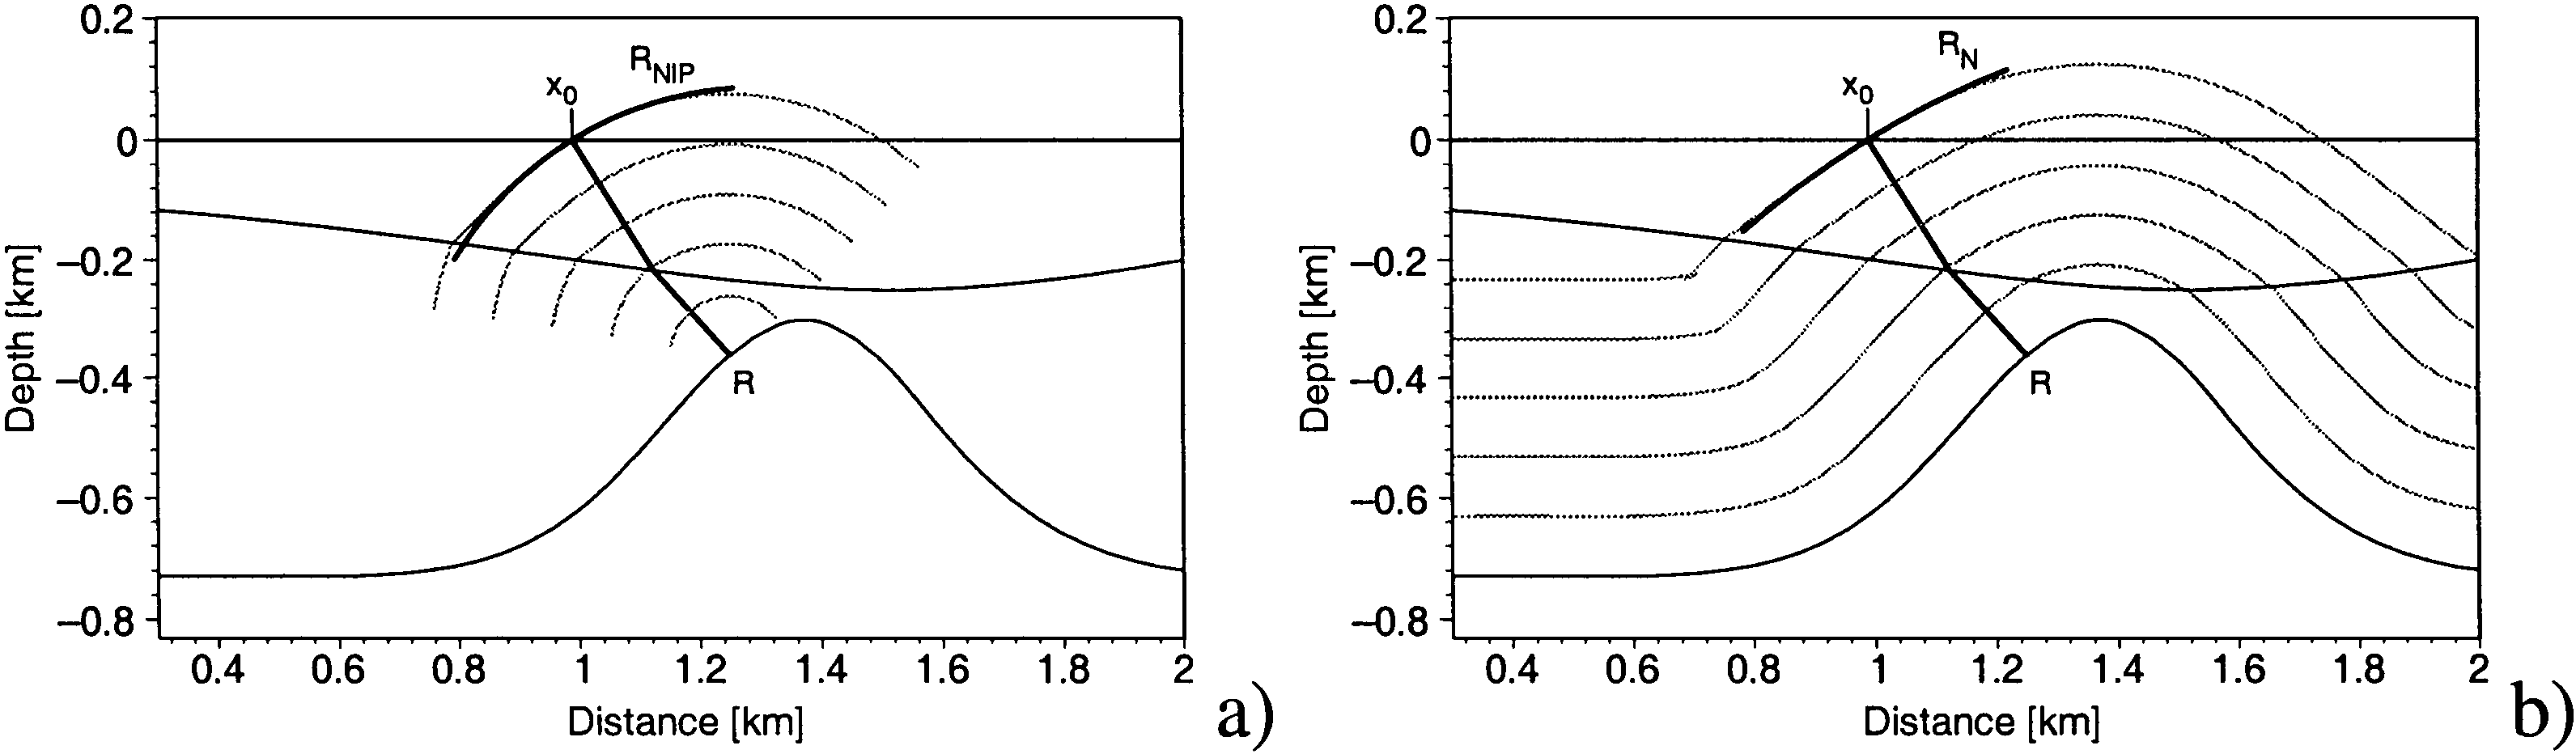
\includegraphics[scale=0.13]{images/crr.png}
\vspace{-0.3cm}
\end{center}
\begin{center}
 Fonte: Jager et al (2001).
\end{center}
\label{fig:3.1}
\end{figure}

O empilhamento CRS assume a seguinte forma:
Assumindo que os dados multicobertura são adquiridos em uma linha sísmica horizontal. Nesta linha, nós consideramos
uma reflexão primária de afastamento nulo fixa ou um raio central. Este raio é especificado a partir da coordenada $x_0$
que localiza o par fonte receptor correspondente e o ângulo de saída $\beta_0$. Reflexões primárias 
paraxiais são especificadas na vizinhança do raio central pelas coordenadas do ponto médio e do meio afastamento $(x_m,h)$.
O tempo de trânsito duplo do raio central é denotado por $t_0$ \cite{chirajc}.


\begin{equation}
\label{eq:3.1}
 S(t_0,m_0)=\int\int P(t(h,d=m-m_0;t_0)dhdm
\end{equation}


Onde a integral na Equação \ref{eq:3.1} ao redor de $m$ é realizada ao longo de uma vizinhança limitada de
um cmp central arbitrário $m_0$.
A superfície CRS $t(h,d)$ é uma função do
tempo de trânsito, em que $d=m_0-m$, é a distância entre o CMP central $m_0$ e um CMP na vizinhança $m$;
$h=x/2$ é o half-offset.
A superfície CRS $t(h,d)$ é uma aproximação do tempo de trânsito SRC o mais acurada possível. Várias
aproximações de tempo de trânsito SRC foram produzidas na literatura, como a aproximação hiperbólica do SRC
\cite{jager}, aproximação SRC quarta ordem \cite{germam}, aproximação não hiperbólica do SRC \cite{fomel1}
e aproximação do SRC Padé \cite{neves}, cada uma com as suas particularidades e graus de acurácia.

\section{APROXIMAÇÕES HIPERBÓLICA DO SRC}

A aproximação do SRC hiperbólico pode ser justificada como
uma expansão em série de Taylor, até segunda ordem, do quadrado do tempo de trânsito 
ao longo de um raio de referência \cite{fomel1}. A aproximação do CRS hiperbólico \cite{jager}:

\begin{equation}
\label{eq:3.2}
 \theta_{CRS}(h,d;t_0)=\sqrt{F(d)+b_2h^2}
\end{equation}


Onde:

\begin{equation}
\label{eq:3.3}
 F(d)=(t_0+a_1d)^2+a_2d^2
\end{equation}

\begin{equation}
\label{eq:3.4}
 a_1=\frac{2\sin(\beta_0)}{v_0}
\end{equation}

\begin{equation}
\label{eq:3.5}
 a_2=\frac{2\cos^2(\beta_0)t_0}{R_Nv_0}
\end{equation}

\begin{equation}
\label{eq:3.6}
 b_2=\frac{2\cos^2(\beta_0)t_0}{R_{NIP}v_0}
\end{equation}

\section{APROXIMAÇÃO NÃO HIPERBÓLICA DO SRC}

\cite{fomel1} propuseram a seguinte modificação de \ref{eq:3.67} com o intuito de melhorar a acurácia
para grandes offsets e separação entre os CMP's:

\begin{equation}
\label{eq:3.7}
 \Phi_{CRS}(h,d;t_0)=\sqrt{\frac{F(d)+ch^2+\sqrt{F(d-h)F(d+h)}}{2}}
\end{equation}


A Equação \ref{eq:3.7} é chamada equação do CRS não-hiperbólico. O parâmetros 
$a_1$, $a_2$ e $b_2$
do CRS hiperbólico são utilizados na definição
dos parâmetros do SRC não hiperbólico como:

\begin{equation}
\label{eq:3.8}
 c=2b_2+a_1^2-a_2
\end{equation}

\begin{equation}
\label{eq:3.9}
 F(d-h)=(t_0+a_1(d-h))^2+a_2(d-h)^2
\end{equation}

\begin{equation}
\label{eq:3.10}
 F(d+h)=(t_0+a_1(d+h))^2+a_2(d+h)^2
\end{equation}

\section{APROXIMAÇÕES DE QUARTA ORDEM DO SRC}

Com o intuito de aumentar a acurácia do método CRS para offsets longos e CMP's mais distantes do CMP central,
etendeu se o método CRS hiperbólico desenvolvendo 3 expansões 
em série de Taylor quarta ordem para a superfície CRS: 
$t(h,d)$ \textit{parabólica}, $t^2(h,d)$ \textit{hiperbólica} e $(t(h,d)-t_0+\frac{2}{v_0}R_{NIP})^2$
\textit{deslocada}. Chamado CRS quarta ordem, 
essas aproximações dependem dos mesmos parâmetros $v_0$, $R_N$, $R_{NIP}$ e $\beta_0$ do CRS hiperbólico,
porém acrescentam mais termos e qualidade à aproximação \cite{germam}.

\begin{multline}
\label{eq:3.11}
 t(h,d)=t_0+\frac{2\sin(\beta_0)}{v_0}d+\frac{\cos^2(\beta_0)}{v_0R_N}d^2+\frac{\cos^2(\beta_0)}{v_0R_{NIP}}h^2 \\
 -\frac{\sin(\beta_0)\cos^2(\beta_0)}{v_0R_N^2}d^3-\frac{\sin(\beta_0)\cos^2(\beta_0)}{v_0R_{NIP}^2R_N}(2R_{NIP}+R_N)dh^2 \\
 -\frac{\cos^2(\beta_0)}{2v_0R_{NIP}^3R_N^2}[R_{NIP}^2(8\cos^2(\beta_0)-6)+R_{NIP}R_N(5\cos^2(\beta_0)-4) \\
 -2R_N^2\sin^2(\beta_0)]h^2d^2-\frac{\cos^2(\beta_0)(5\cos^2(\beta_0)-4)}{4v_0R_N^3}d^4 \\
 +\frac{\cos^2(\beta_0)(4R_{NIP}\sin^2(\beta_0)-R_N\cos^2(\beta_0))}{4v_0R_{NIP}^3R_N}h^4 
\end{multline}

\begin{multline}
\label{eq:3.12}
 t^2(d,h)=t_0^2+\frac{4t_0\sin(\beta_0)}{v}d+2\frac{vt_0\cos^2(\beta_0)+2R_N\sin^2(\beta_0)}{v^2R_N}d^2+\frac{2t_0\cos^2(\beta_0)}{vR_{NIP}}h^2 \\
+\frac{2\sin(\beta_0)\cos^2(\beta_0)(2R_N-vt_0)}{v^2R_N^2}d^3 \\
+\frac{2\sin(\beta_0)\cos^2(\beta_0)(2R_{NIP}R_N-2vt_0R_{NIP}-vt_0R_N}{v^2R_{NIP}^2R_N})dh^2 \\
+\frac{\cos^2(\beta_0)}{v^2R_{NIP}^3R_N^2}[vt_0R_{NIP}^2(6-8\cos^2(\beta_0))+vt_0R_{NIP}R_N(4-5\cos^2(\beta_0)) \\
+2vt_0R_N^2\sin^2(\beta_0)-4R{NIP}R_N^2\sin^2(\beta_0)+R_{NIP}^2R_N(10\cos^2(\beta_0)-8)]d^2h^2 \\ 
+\frac{\cos^2(\beta_0)(R_N(10\cos^2(\beta_0)-8)+vt_0(4-5\cos^2(\beta_0))}{2v^2R_N^3}d^4 \\
+\frac{\cos^2(\beta_0)(4vt_0R_{NIP}\sin^2(\beta_0)-vt_0R_N\cos^2(\beta_0)+2R_{NIP}R_N\cos^2(\beta_0)}{2v^2R_{NIP}^3R_N}h^4
\end{multline}

\begin{multline}
\label{eq:3.13}
(t(h,d)-t_0+\frac{2}{v}R_{NIP})^2=(\frac{2}{v}R_{NIP})^2+\frac{8R_{NIP}\sin(\beta_0)}{v^2}d+4\frac{R_{NIP}\cos^2(\beta_0)+R_N\sin^2(\beta_0)}{v^2R_N}d^2 \\
+\frac{4\cos^2(\beta_0)}{v^2}h^2+\frac{4\sin(\beta_0)\cos^2(\beta_0)(R_N-R_{NIP}}{v^2R_N^2}d^3-\frac{8\sin(\beta_0)\cos^2(\beta_0)}{v^2R_N}dh^2 \\
+\frac{\cos^2(\beta_0)}{v^2R_N^3}[R_N(5\cos^2(\beta_0)-4)+R_{NIP}(4-5\cos^2(\beta_0))]d^4+\frac{4\cos^2(\beta_0)(3-4\cos^2(\beta_0))}{v^2R_N^2}d^2h^2 \\
+\frac{4\cos^2(\beta_0)\sin^2(\beta_0)}{v^2R_{NIP}R_N}h^4
\end{multline}


\section{APROXIMAÇÕES SRC PADÉ}

As aproximações do SRC quarta ordem dão origem a 6 aproximações de Padé do tempo de trânsito SRC, pois
cada uma das expansões do SRC quarta ordem pode ser expandida em duas aproximações de Padé, uma
no domínio do meio afastamento $h$ (oque equivale a manter $d$ constante e expandir em torno de $h$), e
no domínio da distância em relação ao PMC central $d$ (oque equivale a manter $h$ constante e 
realizar a aproximação de Padé tomando $h$ variável) \cite{neves}.

Para uma série de Taylor na forma; 
os coeficientes $\lambda$'s são constantes e $h$ é variável:

\begin{equation} %eq 7
\label{eq:3.14}
t^2(h) \approx \lambda_0+\lambda_1h^2+\lambda_2h^4+O(h^6)
\end{equation}

O aproximante de Padé [2/2] será dado por \cite{neves}:

\begin{equation} %eq 9
\label{eq:3.15}
 [2/2]=\zeta_1+\frac{h^2\zeta_2}{1+\zeta_3h^2}
\end{equation}

Onde:

\begin{equation}
\label{eq:3.16}
 \zeta_1=\lambda_0 
\end{equation}

\begin{equation}
\label{eq:3.17}
 \zeta_2=\lambda_1
\end{equation}

\begin{equation}
\label{eq:3.18}
 \zeta_3=\frac{-\lambda_2}{\lambda_1}
\end{equation}


Se a série de Taylor é expressa na forma da Equação \ref{eq:3.14}, o aproximante de Padé [2/2] desta série de Taylor 
será dado pela Equação \ref{eq:3.15}.

Para uma série de Taylor na forma; 
os coeficientes $\lambda$'s são constantes e $d$ é variável:

\begin{equation}
\label{eq:3.19}
 t^2(d) \approx \lambda_0+\lambda_1d+\lambda_2d^2+\lambda_3d^3+\lambda_4d^4
\end{equation}

O aproximante de Padé [2/2] será \cite{neves}:
\begin{equation}
\label{eq:3.20}
 [2/2]=\frac{p_0+p_1d+p_2d^2}{q_0+q_1d+q_2d^2}
\end{equation}

Onde:

\begin{equation}
\label{eq:3.21}
q_1=\frac{-\lambda_2-\lambda_3+\lambda_4\lambda_1}{\lambda_2^2-\lambda_3\lambda_1}
\end{equation}

\begin{equation}
\label{eq:3.22}
q_2=\frac{-\lambda_4-\lambda_3q_1}{\lambda_2}
\end{equation}

\begin{equation}
\label{eq:3.23}
 p_0=\lambda_0
\end{equation}

\begin{equation}
\label{eq:3.24}
 p_1=\lambda_1+\lambda_0q_1
\end{equation}

\begin{equation}
\label{eq:3.25}
p_2=\lambda_0q_2+\lambda_1q_1+\lambda_2
\end{equation}

O aproximante de Padé [2/2] da Equação \ref{eq:3.6} não possui uma forma compacta como a Equação \ref{eq:3.2}. 
No entanto, é
dado pela Equação \ref{eq:3.7} em função dos coeficientes $p$'s e `$q$'s nas Equações \ref{eq:3.8}-\ref{eq:3.12} 
que dependem
dos coeficientes da própria série de taylor aproximada (coeficientes $\lambda$'s).

\section{APROXIMAÇÃO PARA $t(h,d)$, EXPANSÃO EM h}
\label{sec:6.1}

A aproximação em série de Taylor quarta ordem da superfície CRS, desenvolvida por \cite{germam}, para $t(h,d)$:

\begin{multline}
\label{eq:6.13}
 t(h,d)=t_0+\frac{2\sin(\beta_0)}{v_0}d+\frac{\cos^2(\beta_0)}{v_0R_N}d^2+\frac{\cos^2(\beta_0)}{v_0R_{NIP}}h^2 \\
 -\frac{\sin(\beta_0)\cos^2(\beta_0)}{v_0R_N^2}d^3-\frac{\sin(\beta_0)\cos^2(\beta_0)}{v_0R_{NIP}^2R_N}(2R_{NIP}+R_N)dh^2 \\
 -\frac{\cos^2(\beta_0)}{2v_0R_{NIP}^3R_N^2}[R_{NIP}^2(8\cos^2(\beta_0)-6)+R_{NIP}R_N(5\cos^2(\beta_0)-4) \\
 -2R_N^2\sin^2(\beta_0)]h^2d^2-\frac{\cos^2(\beta_0)(5\cos^2(\beta_0)-4)}{4v_0R_N^3}d^4 \\
 +\frac{\cos^2(\beta_0)(4R_{NIP}\sin^2(\beta_0)-R_N\cos^2(\beta_0))}{4v_0R_{NIP}^3R_N}h^4 
\end{multline}

A variável onde será realizada a aproximação de Padé é $h=x/2$,
$d$ é mantido constante, e a aproximação de Padé [2/2] é realizada somente em $h$.
Definindo os coeficientes $\lambda$'s na forma:

\begin{equation}
\label{eq:6.14}
 \lambda_0=t_0+\frac{2\sin(\beta_0)}{v_0}d+\frac{\cos^2(\beta_0)}{v_0R_N}d^2-\frac{\sin(\beta_0)\cos^2(\beta_0)}{v_0R_N^2}d^3-\frac{\cos^2(\beta_0)(5\cos^2(\beta_0)-4)}{4v_0R_N^3}d^4
\end{equation}

\begin{multline}
\label{eq:6.15}
 \lambda_1=\frac{\cos^2(\beta_0)}{v_0R_{NIP}}-\frac{\sin(\beta_0)\cos^2(\beta_0)}{v_0R_{NIP}^2R_N}(2R_{NIP}+R_N)d \\
  -\frac{\cos^2(\beta_0)}{2v_0R_{NIP}^3R_N^2}[R_{NIP}^2(8\cos^2(\beta_0)-6)+R_{NIP}R_N(5\cos^2(\beta_0)-4)-2R_N^2\sin^2(\beta_0)]d^2
\end{multline}

\begin{equation}
\label{eq:6.16}
  \lambda_2=\frac{\cos^2(\beta_0)(4R_{NIP}\sin^2(\beta_0)-R_N\cos^2(\beta_0))}{4v_0R_{NIP}^3R_N}
\end{equation}

\begin{equation}
\label{eq:6.17}
  \frac{-\lambda_2}{\lambda_1}=-\frac{1}{2}\frac{Q_1}{Q_2}       
\end{equation}

Onde:

\begin{equation}
\label{eq:6.18}
Q_1=4R_{NIP}R_N\sin^2(\beta_0)-R_N^2\cos^2(\beta_0)
\end{equation}


\begin{multline}
\label{eq:6.19}
Q_2=2R_{NIP}^2R_N^2-2R_{NIP}R_N(2R_{NIP}+R_N)\sin(\beta_0)d \\
-[R_{NIP}^2(8\cos^2(\beta_0)-6)+R_{NIP}R_N(5\cos^2(\beta_0)-4)-2R_N^2\sin^2(\beta_0)]d^2
\end{multline}

Definindo os coeficientes $lambda$'s dessa forma, a Equação \ref{eq:3.13} se torna semelhante a
Equação \ref{eq:3.1}. Portanto,
o aproximante de Padé [2/2] da Equação \ref{eq:3.13} será dado também pela Equação \ref{eq:3.2}.

Substituimos os coeficientes $\lambda$'s definidos em \ref{eq:3.14}-\ref{eq:3.17} na definição dos coeficientes $\zeta$'s
nas Equações \ref{eq:3.3}-\ref{eq:3.5}:

\begin{equation}
\label{eq:6.20}
 \zeta_1=\lambda_0=t_0+\frac{2\sin(\beta_0)}{v_0}d+\frac{\cos^2(\beta_0)}{v_0R_N}d^2-\frac{\sin(\beta_0)\cos^2(\beta_0)}{v_0R_N^2}d^3-\frac{\cos^2(\beta_0)(5\cos^2(\beta_0)-4)}{4v_0R_N^3}d^4 
\end{equation}

\begin{multline}
\label{eq:6.21}
 \zeta_2=\lambda_1=\frac{\cos^2(\beta_0)}{v_0R_{NIP}}-\frac{\sin(\beta_0)\cos^2(\beta_0)}{v_0R_{NIP}^2R_N}(2R_{NIP}+R_N)d \\
  -\frac{\cos^2(\beta_0)}{2v_0R_{NIP}^3R_N^2}[R_{NIP}^2(8\cos^2(\beta_0)-6)+R_{NIP}R_N(5\cos^2(\beta_0)-4)-2R_N^2\sin^2(\beta_0)]d^2
\end{multline}

\begin{equation}
\label{eq:6.22}
 \zeta_3=\frac{-\lambda_2}{\lambda_1}=-\frac{1}{2}\frac{Q_1}{Q_2}  
\end{equation}


O aproximante de Padé [2/2] para $t(h,d)$ será dado pela Equação \ref{eq:3.1},
utilizando os coeficientes $\zeta$'s definidos nas Equações \ref{eq:3.20}-\ref{eq:3.22}, 
obtidos a partir dos coeficientes 
$lambda$'s definidos nas Equações \ref{eq:3.14}-\ref{eq:3.17}.

\section{APROXIMAÇÃO PARA $t^2(h,d)$, EXPANSÃO EM h}
\label{sec:6.2}

A aproximação em série de Taylor quarta ordem da superfície CRS, desenvolvida por \cite{germam}, para $t^2(h,d)$:


\begin{multline}
\label{eq:6.23}
 t^2(d,h)=t_0^2+\frac{4t_0\sin(\beta_0)}{v}d+2\frac{vt_0\cos^2(\beta_0)+2R_N\sin^2(\beta_0)}{v^2R_N}d^2+\frac{2t_0\cos^2(\beta_0)}{vR_{NIP}}h^2 \\
+\frac{2\sin(\beta_0)\cos^2(\beta_0)(2R_N-vt_0)}{v^2R_N^2}d^3 \\
+\frac{2\sin(\beta_0)\cos^2(\beta_0)(2R_{NIP}R_N-2vt_0R_{NIP}-vt_0R_N}{v^2R_{NIP}^2R_N})dh^2 \\
+\frac{\cos^2(\beta_0)}{v^2R_{NIP}^3R_N^2}[vt_0R_{NIP}^2(6-8\cos^2(\beta_0))+vt_0R_{NIP}R_N(4-5\cos^2(\beta_0)) \\
+2vt_0R_N^2\sin^2(\beta_0)-4R{NIP}R_N^2\sin^2(\beta_0)+R_{NIP}^2R_N(10\cos^2(\beta_0)-8)]d^2h^2 \\ 
+\frac{\cos^2(\beta_0)(R_N(10\cos^2(\beta_0)-8)+vt_0(4-5\cos^2(\beta_0))}{2v^2R_N^3}d^4 \\
+\frac{\cos^2(\beta_0)(4vt_0R_{NIP}\sin^2(\beta_0)-vt_0R_N\cos^2(\beta_0)+2R_{NIP}R_N\cos^2(\beta_0)}{2v^2R_{NIP}^3R_N}h^4
\end{multline}

A variável onde será realizada a aproximação é $h=x/2$,
$d$ é mantido constante, e a aproximação de Padé [2/2] é realizada somente em $h$.
Definindo os coeficientes $\lambda$'s na forma:

\begin{multline}
\label{eq:6.24}
 \lambda_0=t_0^2+\frac{4t_0\sin(\beta_0)}{V}d+2\frac{Vt_0\cos^2(\beta_0)+2R_N\sin^2(\beta_0)}{V^2R_N}d^2 \\
+\frac{2\sin(\beta_0)\cos^2(\beta_0)(2R_N-Vt_0)}{V^2R_N^2}d^3 \\
+\frac{\cos^2(\beta_0)(R_N(10\cos^2(\beta_0)-8)+Vt_0(4-5\cos^2(\beta_0))}{2V^2R_N^3}d^4 
 \end{multline}
 
\begin{multline}
\label{eq:6.25}
 \lambda_1=\frac{2t_0\cos^2(\beta_0)}{VR_{NIP}}+\frac{2\sin(\beta_0)\cos^2(\beta_0)(2R_{NIP}R_N-2Vt_0R_{NIP}-Vt_0R_N)}{V^2R_{NIP}^2R_N}d \\
+\frac{\cos^2(\beta_0)}{V^2R_{NIP}^3R_N^2}[Vt_0R_{NIP}^2(6-8\cos^2(\beta_0))+Vt_0R_{NIP}R_N(4-5\cos^2(\beta_0)) \\
+2Vt_0R_N^2\sin^2(\beta_0)-4R_{NIP}R_N^2\sin^2(\beta_0)+R_{NIP}^2R_N(10\cos^2(\beta_0)-8)]d^2
\end{multline}

\begin{equation}
\label{eq:6.26}
\lambda_2=\frac{\cos^2(\beta_0)(4Vt_0R_{NIP}\sin^2(\beta_0)-Vt_0R_N\cos^2(\beta_0)+2R_{NIP}R_N\cos^2(\beta_0)}{2V^2R_{NIP}^3R_N}
\end{equation}

\begin{equation}
\label{eq:6.27}
 [-\lambda_2/\lambda_1]=\frac{-R_NQ_3}{2}\frac{1}{(2Vt_0R_{NIP}^2R_N^2+2R_{NIP}R_NQ_1\sin(\beta_0)d+Q_2d^2)}
\end{equation}

Os coeficientes geométricos $Q$'s na Equação \ref{eq:3.27} são:

\begin{equation}
\label{eq:6.28}
 Q_1=2R_{NIP}R_N-2Vt_0R_{NIP}-Vt_0R_N
\end{equation}

\begin{multline}
\label{eq:6.29}
 Q_2=Vt_0R_{NIP}^2(6-8\cos^2(\beta_0))+Vt_0R_{NIP}R_N(4-5\cos^2(\beta_0)) \\
 +2Vt_0R_N^2\sin^2(\beta_0)-4R{NIP}R_N^2\sin^2(\beta_0)+R_{NIP}^2R_N(10\cos^2(\beta_0)-8)
\end{multline}

\begin{equation}
\label{eq:6.30}
 Q_3=4Vt_0R_{NIP}\sin^2(\beta_0)-Vt_0R_N\cos^2(\beta_0)+2R_{NIP}R_N\cos^2(\beta_0)
\end{equation}

Definindo os coeficientes $\lambda$'s dessa forma, a Equação \ref{eq:3.23} se torna semelhante a
Equação \ref{eq:3.1}. Portanto,
o aproximante de Padé [2/2] da Equação \ref{eq:3.23} será dado também por \ref{eq:3.2}.

Substituimos os coeficientes $\lambda$'s definidos nas Equações
\ref{eq:3.25}-\ref{eq:3.27} na definição dos coeficientes $\zeta$'s
em \ref{eq:3.3}-\ref{eq:3.5}:

\begin{multline}
\label{eq:6.31}
 \zeta_1=\lambda_0=t_0^2+\frac{4t_0\sin(\beta_0)}{V}d+2\frac{Vt_0\cos^2(\beta_0)+2R_N\sin^2(\beta_0)}{V^2R_N}d^2 \\
+\frac{2\sin(\beta_0)\cos^2(\beta_0)(2R_N-Vt_0)}{V^2R_N^2}d^3 \\
+\frac{\cos^2(\beta_0)(R_N(10\cos^2(\beta_0)-8)+Vt_0(4-5\cos^2(\beta_0))}{2V^2R_N^3}d^4 
\end{multline}

\begin{multline}
\label{eq:6.32}
 \zeta_2=\lambda_1=\frac{2t_0\cos^2(\beta_0)}{VR_{NIP}}+\frac{2\sin(\beta_0)\cos^2(\beta_0)(2R_{NIP}R_N-2Vt_0R_{NIP}-Vt_0R_N)}{V^2R_{NIP}^2R_N}d \\
+\frac{\cos^2(\beta_0)}{V^2R_{NIP}^3R_N^2}[Vt_0R_{NIP}^2(6-8\cos^2(\beta_0))+Vt_0R_{NIP}R_N(4-5\cos^2(\beta_0)) \\
+2Vt_0R_N^2\sin^2(\beta_0)-4R_{NIP}R_N^2\sin^2(\beta_0)+R_{NIP}^2R_N(10\cos^2(\beta_0)-8)]d^2
\end{multline}

\begin{equation}
\label{eq:6.33}
 \zeta_3=\frac{-\lambda_2}{\lambda_1}=\frac{-R_NQ_3}{2}\frac{1}{(2Vt_0R_{NIP}^2R_N^2+2R_{NIP}R_NQ_1\sin(\beta_0)d+Q_2d^2)} 
\end{equation}


O aproximante de Padé [2/2] para $t^2(h,d)$ será dado pela Equação \ref{eq:3.2},
utilizando os coeficientes $\zeta$'s definidos nas Equações \ref{eq:3.31}-\ref{eq:3.33}, 
obtidos a partir dos coeficientes 
$\lambda$'s definidos nas Equações \ref{eq:3.24}-\ref{eq:3.27}.


\section{APROXIMAÇÃO PARA $(t(d,h)-t_0+\frac{2}{v}R_{NIP})^2$, EXPANSÃO EM h}
\label{sec:6.3}
A aproximação em série de Taylor quarta ordem da superfície CRS, 
desenvolvida por \cite{germam}, para $(t(h,d)-t_0+\frac{2}{v}R_{NIP})^2$:

\begin{multline}
\label{eq:6.34}
(t(h,d)-t_0+\frac{2}{v}R_{NIP})^2=(\frac{2}{v}R_{NIP})^2+\frac{8R_{NIP}\sin(\beta_0)}{v^2}d+4\frac{R_{NIP}\cos^2(\beta_0)+R_N\sin^2(\beta_0)}{v^2R_N}d^2 \\
+\frac{4\cos^2(\beta_0)}{v^2}h^2+\frac{4\sin(\beta_0)\cos^2(\beta_0)(R_N-R_{NIP}}{v^2R_N^2}d^3-\frac{8\sin(\beta_0)\cos^2(\beta_0)}{v^2R_N}dh^2 \\
+\frac{\cos^2(\beta_0)}{v^2R_N^3}[R_N(5\cos^2(\beta_0)-4)+R_{NIP}(4-5\cos^2(\beta_0))]d^4+\frac{4\cos^2(\beta_0)(3-4\cos^2(\beta_0))}{v^2R_N^2}d^2h^2 \\
+\frac{4\cos^2(\beta_0)\sin^2(\beta_0)}{v^2R_{NIP}R_N}h^4
\end{multline}

A variável onde será realizada a aproximação é $h=x/2$,
$d$ é mantido constante, e a aproximação de Padé [2/2] é realizada somente em $h$.
Definindo os coeficientes $\lambda$'s na forma:

\begin{multline}
\label{eq:6.35}
 \lambda_0=(\frac{2}{v_0}R_{NIP})^2+\frac{8R_{NIP}\sin(\beta_0)}{v_0^2}d+4\frac{R_NIP\cos^2(\beta_0)+R_N\sin^2(\beta_0)}{v_0^2R_N}d^2 \\
 +\frac{4\sin(\beta_0)\cos^2(\beta_0)(R_N-R_{NIP}}{v_0^2R_N^2}d^3 \\
 +\frac{\cos^2(\beta_0)}{v_0^2R_N^3}[R_N(5\cos^2(\beta_0)-4)+R_{NIP}(4-5\cos^2(\beta_0))]d^4
 \end{multline}
 
\begin{equation}
\label{eq:6.36}
 \lambda_1=\frac{4\cos^2(\beta_0)}{v_0^2}-\frac{8\sin(\beta_0)\cos^2(\beta_0)}{v_0^2R_N}d+\frac{4\cos^2(\beta_0)(3-4\cos^2(\beta_0))}{v_0^2R_N^2}d^2
\end{equation}

\begin{equation}
\label{eq:6.37}
\lambda_2=\frac{4\cos^2(\beta_0)\sin^2(\beta_0)}{v_0^2R_{NIP}R_N}
\end{equation}

\begin{equation}
\label{eq:6.38}
 [-\lambda_2/\lambda_1]=-\frac{R_N\sin^2(\beta_0)}{R_{NIP}}\frac{1}{R_N^2-2R_N\sin(\beta_0)d+(3-4\cos^2(\beta_0))d^2}
\end{equation}

Definindo os coeficientes $\lambda$'s dessa forma, a Equação \ref{eq:3.34} se torna semelhante a
Equação \ref{eq:3.1}. Portanto,
o aproximante de Padé [2/2] da Equação \ref{eq:3.34} será dado também pela Equação \ref{eq:3.2}.

Substituimos os coeficientes $\lambda$'s definidos em \ref{eq:3.35}-\ref{eq:3.38} na definição dos coeficientes $\zeta$'s
nas Equações \ref{eq:3.3}-\ref{eq:3.5}:

\begin{multline}
\label{eq:6.39}
 \zeta_1=\lambda_0=(\frac{2}{v_0}R_{NIP})^2+\frac{8R_{NIP}\sin(\beta_0)}{v_0^2}d+4\frac{R_NIP\cos^2(\beta_0)+R_N\sin^2(\beta_0)}{v_0^2R_N}d^2 \\
 +\frac{4\sin(\beta_0)\cos^2(\beta_0)(R_N-R_{NIP}}{v_0^2R_N^2}d^3 \\
 +\frac{\cos^2(\beta_0)}{v_0^2R_N^3}[R_N(5\cos^2(\beta_0)-4)+R_{NIP}(4-5\cos^2(\beta_0))]d^4
\end{multline}

\begin{equation}
\label{eq:6.40}
 \zeta_2=\lambda_1=\frac{4\cos^2(\beta_0)}{v_0^2}-\frac{8\sin(\beta_0)\cos^2(\beta_0)}{v_0^2R_N}d+\frac{4\cos^2(\beta_0)(3-4\cos^2(\beta_0))}{v_0^2R_N^2}d^2
\end{equation}

\begin{equation}
\label{eq:6.41}
 \zeta_3=\frac{-\lambda_2}{\lambda_1}=-\frac{R_N\sin^2(\beta_0)}{R_{NIP}}\frac{1}{R_N^2-2R_N\sin(\beta_0)d+(3-4\cos^2(\beta_0))d^2} 
\end{equation}

O aproximante de Padé [2/2] para $(t(h,d)-t_0+\frac{2}{v}R_{NIP})^2$ será dado pela Equação \ref{eq:3.2},
utilizando os coeficientes $\zeta$'s definidos nas Equações \ref{eq:3.39}-\ref{eq:3.41}, a partir dos coeficientes 
$\lambda$'s definidos em \ref{eq:3.35}-\ref{eq:3.38}.

\section{APROXIMAÇÃO PARA $t(h,d)$, EXPANSÃO EM d}
\label{sec:6.4}
A variável onde será realizada a expansão é $d=m-mo$, 
para tanto $h$ é mantido constante e a aproximação de Padé {2/2] é realizada somente em $d$.
Se definimos os coeficientes $\lambda$'s na Equação \ref{eq:3.14} de modo que esta se torne semelhante 
a Equação \ref{eq:3.6},
o aproximante de Padé [2/2] da Equação \ref{eq:3.14} será dado pela Equação \ref{eq:3.7}.
Definindo os coeficientes $\lambda$'s da aproximação em série de Taylor quarta ordem da superfície CRS, 
desenvolvida por \cite{germam}, para $t(h,d)$ (Equação \ref{eq:3.14}):

%Definição dos coeficientes
\begin{equation}
\label{eq:6.42}
 \lambda_0=t_0+\frac{\cos^2(\beta_0)}{v_0R_{NIP}}h^2+\frac{\cos^2(\beta_0)(4R_{NIP}\sin^2(\beta_0)-R_N\cos^2(\beta_0))}{4v_0R_{NIP}^3R_N}h^4 
 \end{equation}
 
\begin{equation}
\label{eq:6.43}
 \lambda_1=\frac{2\sin(\beta_0)}{v_0}-\frac{\sin(\beta_0)\cos^2(\beta_0)}{v_0R_{NIP}^2R_N}(2R_{NIP}+R_N)h^2  
\end{equation}

\begin{multline}
\label{eq:6.44}
\lambda_2=\frac{\cos^2(\beta_0)}{v_0R_N}-\frac{\cos^2(\beta_0)}{2v_0R_{NIP}^3R_N^2}[R_{NIP}^2(8\cos^2(\beta_0)-6) \\
 +R_{NIP}R_N(5\cos^2(\beta_0)-4)-2R_N^2\sin^2(\beta_0)]h^2
\end{multline}

\begin{equation}
\label{eq:6.45}
\lambda_3=-\frac{\sin(\beta_0)\cos^2(\beta_0)}{v_0R_N^2}
\end{equation}

\begin{equation}
\label{eq:6.46}
\lambda_4=-\frac{\cos^2(\beta_0)(5\cos^2(\beta_0)-4)}{4v_0R_N^3}
\end{equation}

O aproximante de Padé será dado pela Equação \ref{eq:3.7}:
Os coeficientes dos polinômios $p(d)$ e $q(d)$ são obtidos por meio de \ref{eq:3.8}-\ref{eq:3.12},
utilizando os coeficientes $\lambda$'s definidos nas Equações \ref{eq:3.42}-\ref{eq:3.46}.

\section{APROXIMAÇÃO PARA $t^2(h,d)$, EXPANSÃO EM d}
\label{sec:6.5}
A variável onde será realizada a aproximação de Padé [2/2] é $d=m-mo$, 
para tanto $h$ é mantido constante e a aproximação de Padé é realizada somente em $d$.
Se definimos os coeficientes $\lambda$'s na Equação \ref{eq:3.23} de modo que esta se torne semelhante à \ref{eq:3.6},
o aproximante de Padé [2/2] da Equação \ref{eq:3.23} será dado por \ref{eq:3.7}.
Definindo os coeficientes $\lambda$'s da aproximação em série de Taylor quarta ordem da superfície CRS, 
desenvolvida por \cite{germam}, para $t^2(h,d)$ (\ref{eq:3.23}):

%Definição dos coeficientes
\begin{multline}
\label{eq:6.47}
 \lambda_0=t_0^2+\frac{2h^2t_0\cos^2(\beta_0)}{v_0R_{NIP}} \\
 +\frac{h^4\cos^2(\beta_0)(4v_0t_0R_{NIP}\sin^2(\beta_0)-v_0t_0R_N\cos^2(\beta_0)+2R_{NIP}R_N\cos^2(\beta_0))}{2v_0^2R_{NIP}^3R_N}
 \end{multline}
 
\begin{equation}
\label{eq:6.48}
 \lambda_1=\frac{4t_0\sin(\beta_0)}{v_0}+\frac{2\sin(\beta_0)\cos^2(\beta_0)(2R_{NIP}R_N-2v_0toR_{NIP}-v_0t_0R_N)h^2}{v_0^2R_{NIP}^2R_N}
\end{equation}

\begin{multline}
\label{eq:6.49}
\lambda_2=\frac{2(v_0t_0\cos^2(\beta_0)+2R_N\sin^2(\beta_0)}{v_0^2R_N} \\
+\frac{\cos^2(\beta_0)}{v_0^2R_{NIP}^3R_N^2}[v_0t_0R_{NIP}^2(6-8\cos^2(\beta_0))+v_0t_0R_{NIP}R_N(4-5\cos^2(\beta_0)) \\
+2v_0t_0R_N^2\sin^2(\beta_0)-4R_{NIP}R_N^2\sin^2(\beta_0)+R_{NIP}^2R_N(10\cos(\beta_0)-8)]h^2
\end{multline}

\begin{equation}
\label{eq:6.50}
\lambda_3=\frac{2\sin(\beta_0)\cos^2(\beta_0)(2R_N-v_0t_0)}{v_0^2R_N^2}
\end{equation}

\begin{equation}
\label{eq:6.51}
\lambda_4=\frac{\cos^2(\beta_0)(R_N(10\cos^2(\beta_0)-8)+v_0t_0(4-5\cos^2(\beta_0))}{2v_0^2R_N^3}
\end{equation}

O aproximante de Padé [2/2] será dado pela Equação \ref{eq:3.7}:
Os coeficientes dos polinômios $p(d)$ e $q(d)$ são obtidos por meio das Equações \ref{eq:3.8}-\ref{eq:3.12},
utilizando os coeficientes $\lambda$'s definidos nas Equações \ref{eq:3.47}-\ref{eq:3.51}.

\section{APROXIMAÇÃO PARA $(t(h,d)-t_0+\frac{2}{v_0}R_{NIP})^2$, EXPANSÃO EM d}
\label{sec:6.6}
A variável onde será realizada a aproximação de Padé [2/2] é $d=m-mo$, 
para tanto $h$ é mantido constante e a aproximação de Padé é realizada somente em $d$.
Se definimos os coeficientes $\lambda$'s na Equação \ref{eq:3.34} de modo que esta se torne semelhante 
a Equação \ref{eq:3.6},
o aproximante de Padé [2/2] da Equação \ref{eq:3.34} será dado por \ref{eq:3.7}.
Definindo os coeficientes $\lambda$'s da aproximação em série de Taylor quarta ordem da superfície CRS, 
desenvolvida por \cite{germam}, para $(t(d,h)-t_0+\frac{2}{v_0}R_{NIP})^2$ (Equação \ref{eq:5.34}):

%Definição dos coeficientes
\begin{equation}
\label{eq:6.52}
 \lambda_0=(\frac{2}{v_0}R_{NIP})^2+\frac{4\cos^2(\beta_0)}{v_0^2}h^2+\frac{4\cos^2(\beta_0)\sin^2(\beta_0)}{v_0^2R_{NIP}R_N}h^4
 \end{equation}
 
\begin{equation}
\label{eq:6.53}
 \lambda_1=\frac{8R_{NIP}\sin(\beta_0)}{v_0^2}-\frac{8\sin(\beta_0)\cos^2(\beta_0)}{v_0^2R_N}h^2 
\end{equation}

\begin{equation}
\label{eq:6.54}
\lambda_2=4\frac{R_NIP\cos^2(\beta_0)+R_N\sin^2(\beta_0)}{v_0^2R_N}+\frac{4\cos^2(\beta_0)(3-4\cos^2(\beta_0))}{v_0^2R_N^2}h^2
\end{equation}

\begin{equation}
\label{eq:6.55}
\lambda_3=\frac{4\sin(\beta_0)\cos^2(\beta_0)(R_N-R_{NIP}}{v_0^2R_N^2}
\end{equation}

\begin{equation}
\label{eq:6.56}
\lambda_4=\frac{\cos^2(\beta_0)}{v_0^2R_N^3}[R_N(5\cos^2(\beta_0)-4)+R_{NIP}(4-5\cos^2(\beta_0))]
\end{equation}


O aproximante de Padé [2/2] será dado pela Equação \ref{eq:3.7}:
Os coeficientes dos polinômios $p(d)$ e $q(d)$ são obtidos por meio das Equações \ref{eq:3.8}-\ref{eq:3.12},
utilizando os coeficientes $\lambda$'s definidos nas Equações \ref{eq:3.52}-\ref{eq:3.56}.



 %CRS
% \chapter{CRE}
\label{cap4}

Estes parâmetros são atributos específicos de uma frente de onda hipotética atribuídos a cada evento de reflexão
primária de afastamento nulo: O raio de curvatura RNIP e o ângulo de emergência $\beta_0$. Esta onda hipotética é
a onda NIP (Hubral, 1983)

Hubral, P.
Computing true-amplitude reflections in a laterally inhomogeneous earth
Geophysics 48 1052-1063



O método do elemento de reflexão comum (CRE) é uma alternativa interessante para os métodos usuais de empilhamento PMC ou
migração para a seção de afastamento nulo. No entanto não requere conhecimento do modelo geral em subsuperfície, apenas
o conhecimento da velocidade próximo a superfície é necessário a priori.
O método ERC é baseado somente em considerações cinemáticas em 2D e não é
um processo que preserva as amplitudes.

A principal e provavelmente mais importante vantagem do método ERC em comparação com o empilhamento PMC convencional
é que este proporciona, além da seção empilhada, parâmetros importantes para a construção do macromodelo de 
velocidades que pode inclusive variar lateralmente.

Os parâmetros $R_{NIP}$ e $\beta_0$ atribuídos aos pontos $P_0(x_0,\tau_0)$ são obtidos a partir do método ERC.
Estes dois atributos podem ser utilizados para estimar o macromodelo de velocidades.
O método ERC, além de ser um processo para simular as seções de afastamento nulo sem o conhecimento prévio
do macromodelo de velocidades, também permite determinar os atributos da onda NIP $(R_{NIP},\beta_0)$
que combinado com outras estratégias permitem estimar o macromodelo de velocidades.

As principais características do método ERC:
(a) A construção da seção de afastamento nulo a partir de um conjunto de seções de afastamento constante
com apenas uma estimativa da velocidade próxima da superfície.
(b) A determinação dos parâmetros $(R_{NIP},\beta_0)$ para as reflexões de afastamento nulo na seção empilhada.
Estes atributos podem ser utilizados com técnicas de inversão para estimar o macromodelo de velocidades.

A idéia principal do método ERC é, usando a fórmula do tempo de trânsito ERC, no modelo auxiliar, dado um intervalo
de busca para os parâmetros $R_{NIP}$ e $\beta_0$, encontrar a frente de onda NIP que melhor se ajusta aos dados.
Este processo é semelhante a análise sobretempo normal convencional, todavia enquanto esta análise é feita no
domínio PMC, o método ERC é feito no domínio ERC construído durante o processo, o parâmetro otimizado $R_{NIP}$,$\beta_0$
é especificado a partir da análise de coerência nos dados.


\begin{figure}[htb]
\caption{Representação esquemática de um arranjo ERC para um refletor circular de raio $R$ e profundidade
mínima $D$: A família ERC é formada pelos pares $s_i$-$r_i$ (fonte-receptor) que possuem o mesmo ponto de
reflexão em subsuperfície ($NIP$). A família ERC pode ser entendida a partir de uma fonte pontual explosiva
no ponto $NIP$, que ao ser ativada forma uma frente de onda $NIP$ que atinge a superfície em um PMC central 
$m_0$ com raio de curvatura $R_{NIP}$ e ângulo de incidência $\beta_0$.}
\begin{center}
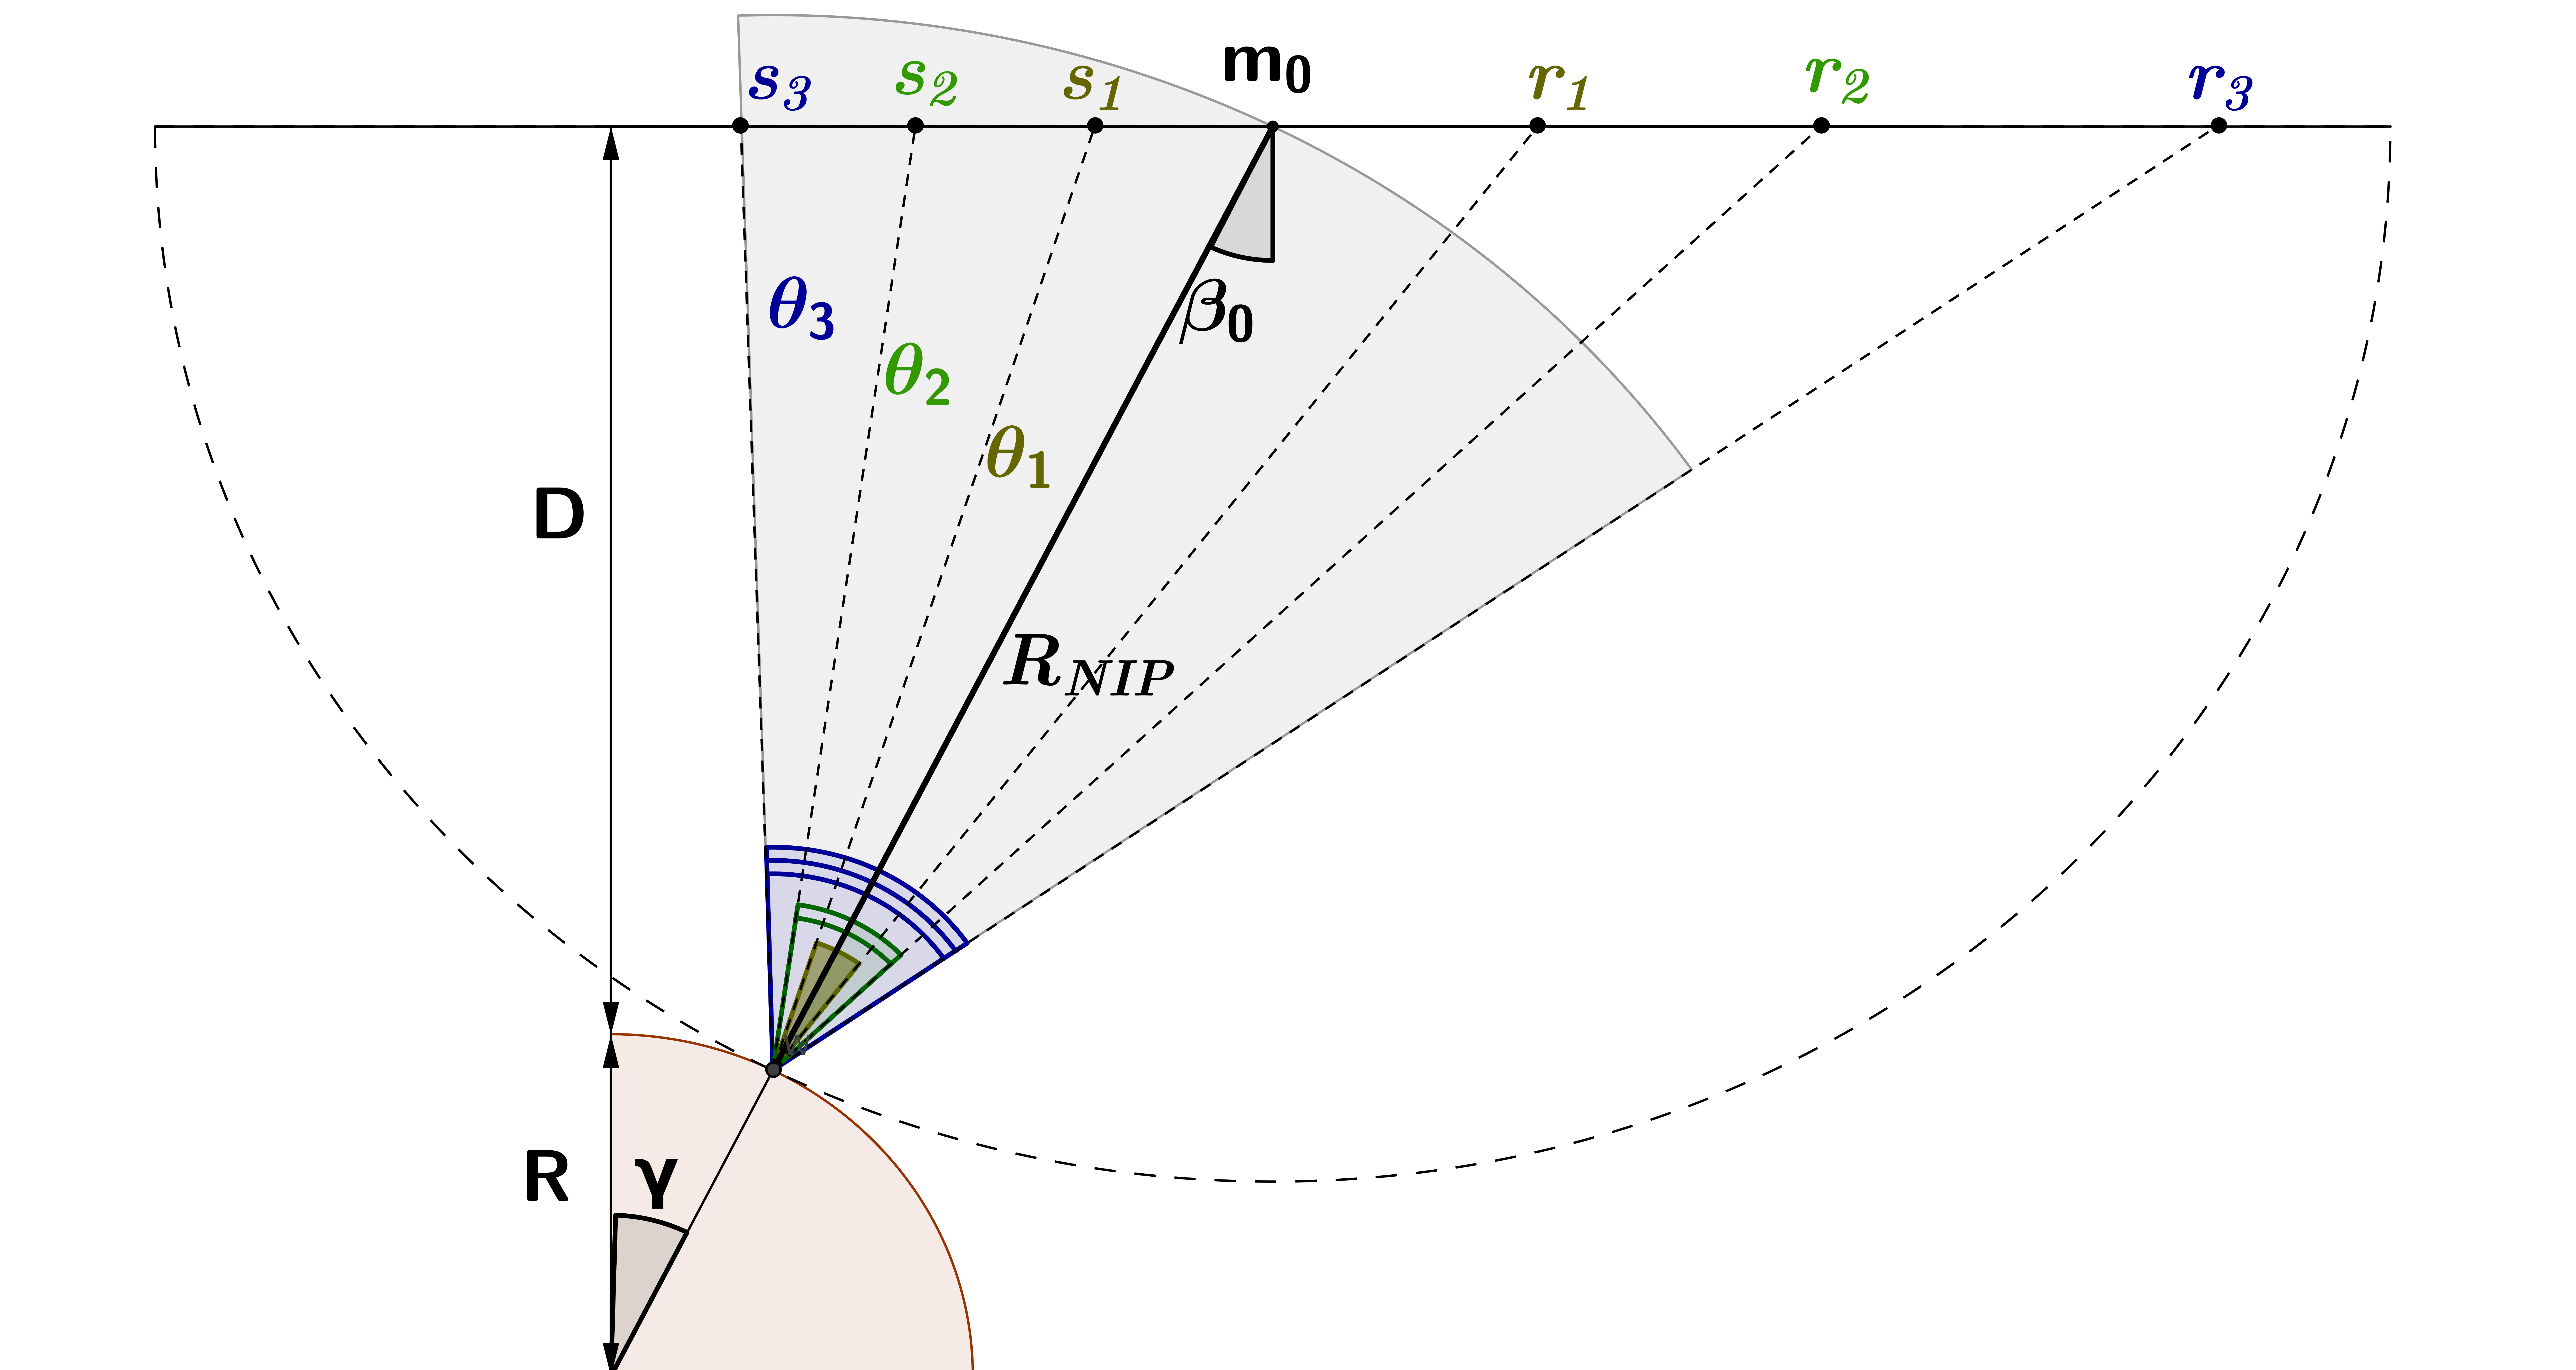
\includegraphics[scale=0.3]{images/cre.png}
\vspace{-0.3cm}
\end{center}
\begin{center}
 Fonte: Do Autor.
\end{center}
\label{fig:4.1}
\end{figure}


\begin{figure}[htb]
\caption{Representação esquemática das coordenadas do ERC sobre o modelo do refletor circular da Figura \ref{fig:4.1}:
Modificamos a posição do PMC central $m_0$ variando o ângulo $\gamma$ no modelo do refletor circular.
Ao variarmos o ângulo $\theta$, mantendo $\gamma$ constante, obtemos os pares $s_i$-$r_i$ (fonte-receptor)
dentro da família
ERC, as posições $h$ (meio afastamento) e $m$ (PMC) são obtidas para cada par fonte-receptor.
Cada curva colorida representa uma posição
diferente de $m_0$, um valor diferente de $R_{NIP}$ e $\beta_0$, e uma família ERC diferente.}
\begin{center}
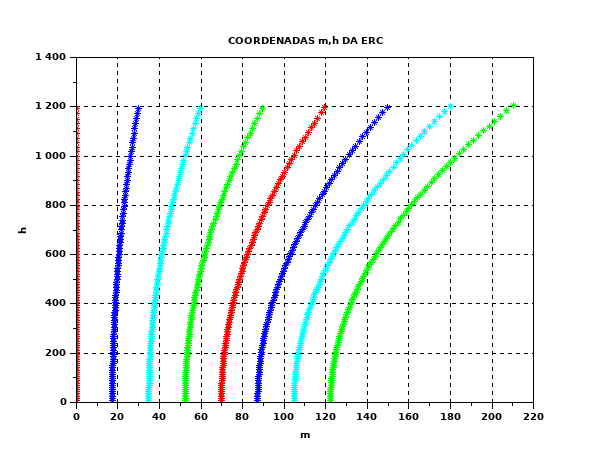
\includegraphics[scale=0.5]{images/coordenadas_CRE.png}
\vspace{-0.3cm}
\end{center}
\begin{center}
 Fonte: Do Autor.
\end{center}
\label{fig:4.2}
\end{figure}





O parâmetro de assimetria desenpenha um papel importante na seleção de pares fonte-receptor para os quais
o correspondente raio de reflexão refletem no mesmo ponto \cite{tygel}.


 %CRE
 \chapter{MODELO DO REFLETOR CIRCULAR E O MÉTODO ERC}
\label{cap7}

Uma maneira bastante didática de entender o empilhamento SRC é partir de um modelo simples,
derivar a superfície de tempo de trânsito SRC em função dos
parâmetros da geometria do modelo:
No caso do modelo do refletor circular,  representado esquematicamente na Figura \ref{fig:7.1}, 
em um meio homogêneo de velocidade $v_0$,
a solução analítica fechada é complicada, pois envolve uma solução de uma equação polinomial de
alta ordem \cite{landa}.
No entanto, a superfície de tempo de trânsito de reflexão pode ser descrita analiticamente por relações paramétricas
\cite{glaeser}.

%figura da hipérbole
\begin{figure}[htb]
\caption{Representação esquemática do modelo do refletor circular de profundidade $D$
em um meio de velocidade constante $v_0$.
$m$ é a posição do ponto médio do par fonte $s$ e receptor $r$, $L=R+D$ é o comprimento do raio normal, 
$\beta_0$ é ângulo de emergência
do raio normal na superfície e $R$ é o raio do refletor circular.}
\begin{flushleft}
\includegraphics[scale=0.45]{images/circ.png}
\vspace{-0.3cm}
\end{flushleft}
\begin{center}
 Fonte: Do Autor.
\end{center}
\label{fig:7.1}
\end{figure}



As coordenadas do ponto médio $m$ e do meio-afastamento $h=x/2$ 
são expressas paramétricamente por:

\begin{equation}
\label{eq:7.1}
 m=R\sin(\gamma)+(D+R-R\cos(\gamma))\frac{\cos(\gamma)\cos(\gamma)}{\cos^2(\theta)-\sin^2(\gamma)}
\end{equation}

\begin{equation}
\label{eq:7.2}
 h=(D+R-R\cos(\gamma))\frac{\cos(\theta)\cos(\theta)}{\cos^2(\theta)-\sin^2(\gamma)}
\end{equation}

\begin{figure}[htb]
\caption{Representação esquemática de um arranjo ERC }
\begin{center}
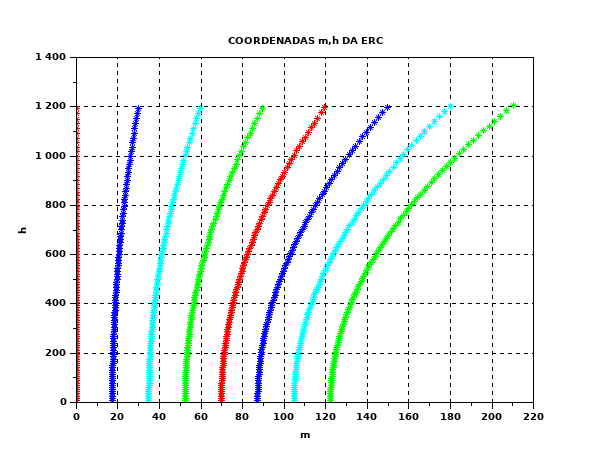
\includegraphics[scale=0.5]{images/coordenadas_CRE.png}
\vspace{-0.3cm}
\end{center}
\begin{center}
 Fonte: Do Autor.
\end{center}
\label{fig:7.2}
\end{figure}


E o tempo de reflexão é expresso como:

\begin{equation}
\begin{flalign*}
\label{eq:7.3}
 \Psi &=\frac{D+R-R\cos(\gamma)}{v_0} \left[ \frac{1}{\cos(\gamma-\theta)}+\frac{1}{\cos(\gamma+\theta)} \right] \\
 &=2\frac{D+R-R\cos(\gamma)}{v_0}\frac{\cos(\gamma)\cos(\theta)}{\cos^2(\theta)-\sin^2(\gamma)}
\end{flalign*} 
\end{equation}


\begin{figure}[htb]
\caption{Representação esquemática do modelo do refletor circular de profundidade $D$
em um meio de velocidade constante $v_0$.
$m$ é a posição do ponto médio do par fonte $s$ e receptor $r$, $L=R+D$ é o comprimento do raio normal, 
$\beta_0$ é ângulo de emergência
do raio normal na superfície e $R$ é o raio do refletor circular.}
\begin{flushleft}
\includegraphics[scale=0.45]{images/circ_mod.png}
\vspace{-0.3cm}
\end{flushleft}
\begin{center}
 Fonte: Do Autor.
\end{center}
\label{fig:7.3}
\end{figure}

Analisnado a Figura \ref{fig:7.1} podemos ver que os parâmetros do SRC podem ser obtidos a partir
de relações trigonométricas simples apliacadas ao triâmgulo retângulo da Figura \ref{fig:7.3}, de cateto menor
$m_0$, cateto maior $L=D+R$ e hipotenusa $R_N=R+R_{NIP}$.
A relação com os parâmetros do SRC é dada analiticamente, em função dos parâmetros do modelo, por:

\begin{equation}
\label{eq:7.4}
t_0=\frac{2(\sqrt{m_0^2+L^2}-R)}{v_0}
\end{equation}

\begin{equation}
\label{eq:7.5}
R_{NIP}=\sqrt{m_0^2+L^2}-R
\end{equation}

\begin{equation}
\label{eq:7.6}
R_N =\sqrt{m_0^2+L^2}
\end{equation}

\begin{equation}
\label{eq:7.7}
\sin(\beta_0)=\frac{m_0}{\sqrt{m_0^2+L^2}}
\end{equation}


As Equações \ref{eq:7.1}-\ref{eq:7.3} definem a superfície de tempo de reflexão $\Psi(h,d)$ pela dependência paramétrica
$\{m(\alpha,\theta),h(\alpha,\theta),\Psi(\alpha,\theta)\}$.
Onde $L=D+R$, $v_0$ é a velocidade do meio, $\beta_0$ é ângulo de emergência
do raio normal, e $m_0$ é o ponto médio central.


\section{ELEMENTO DE REFLEXÃO COMUM (ERC)}

O método do elemento de reflexão comum (CRE) é uma alternativa interessante para os métodos usuais de empilhamento PMC ou
migração para a seção de afastamento nulo. No entanto não requere conhecimento do modelo geral em subsuperfície, apenas
o conhecimento da velocidade próximo a superfície é necessário a priori.
O método ERC é baseado somente em considerações cinemáticas em 2D e não é
um processo que preserva as amplitudes.

A principal e provavelmente mais importante vantagem do método ERC em comparação com o empilhamento PMC convencional
é que este proporciona, além da seção empilhada, parâmetros importantes para a construção do macromodelo de 
velocidades que pode inclusive variar lateralmente.
Estes parâmetros são atributos específicos de uma frente de onda hipotética atribuídos a cada evento de reflexão
primária de afastamento nulo: O raio de curvatura RNIP e o ângulo de emergência $\beta_0$. Esta onda hipotética é
a onda NIP \cite{hubral}.
Os parâmetros $R_{NIP}$ e $\beta_0$ atribuídos aos pontos $P_0(x_0,\tau_0)$ são obtidos a partir do método ERC.
Estes dois atributos podem ser utilizados para estimar o macromodelo de velocidades.
O método ERC, além de ser um processo para simular as seções de afastamento nulo sem o conhecimento prévio
do macromodelo de velocidades, também permite determinar os atributos da onda NIP $(R_{NIP},\beta_0)$
que combinado com outras estratégias permitem estimar o macromodelo de velocidades.

As principais características do método ERC:
(a) A construção da seção de afastamento nulo a partir de um conjunto de seções de afastamento constante
com apenas uma estimativa da velocidade próxima da superfície.
(b) A determinação dos parâmetros $(R_{NIP},\beta_0)$ para as reflexões de afastamento nulo na seção empilhada.
Estes atributos podem ser utilizados com técnicas de inversão para estimar o macromodelo de velocidades.

A idéia principal do método ERC é, usando a fórmula do tempo de trânsito ERC, no modelo auxiliar, dado um intervalo
de busca para os parâmetros $R_{NIP}$ e $\beta_0$, encontrar a frente de onda NIP que melhor se ajusta aos dados.
Este processo é semelhante a análise sobretempo normal convencional, todavia enquanto esta análise é feita no
domínio PMC, o método ERC é feito no domínio ERC construído durante o processo, o parâmetro otimizado $R_{NIP}$,$\beta_0$
é especificado a partir da análise de coerência nos dados.


\begin{figure}[htb]
\caption{Representação esquemática de um arranjo ERC para um refletor circular de raio $R$ e profundidade
mínima $D$: A família ERC é formada pelos pares $s_i$-$r_i$ (fonte-receptor) que possuem o mesmo ponto de
reflexão em subsuperfície ($NIP$). A família ERC pode ser entendida a partir de uma fonte pontual explosiva
no ponto $NIP$, que ao ser ativada forma uma frente de onda $NIP$ que atinge a superfície em um PMC central 
$m_0$ com raio de curvatura $R_{NIP}$ e ângulo de incidência $\beta_0$.}
\begin{center}
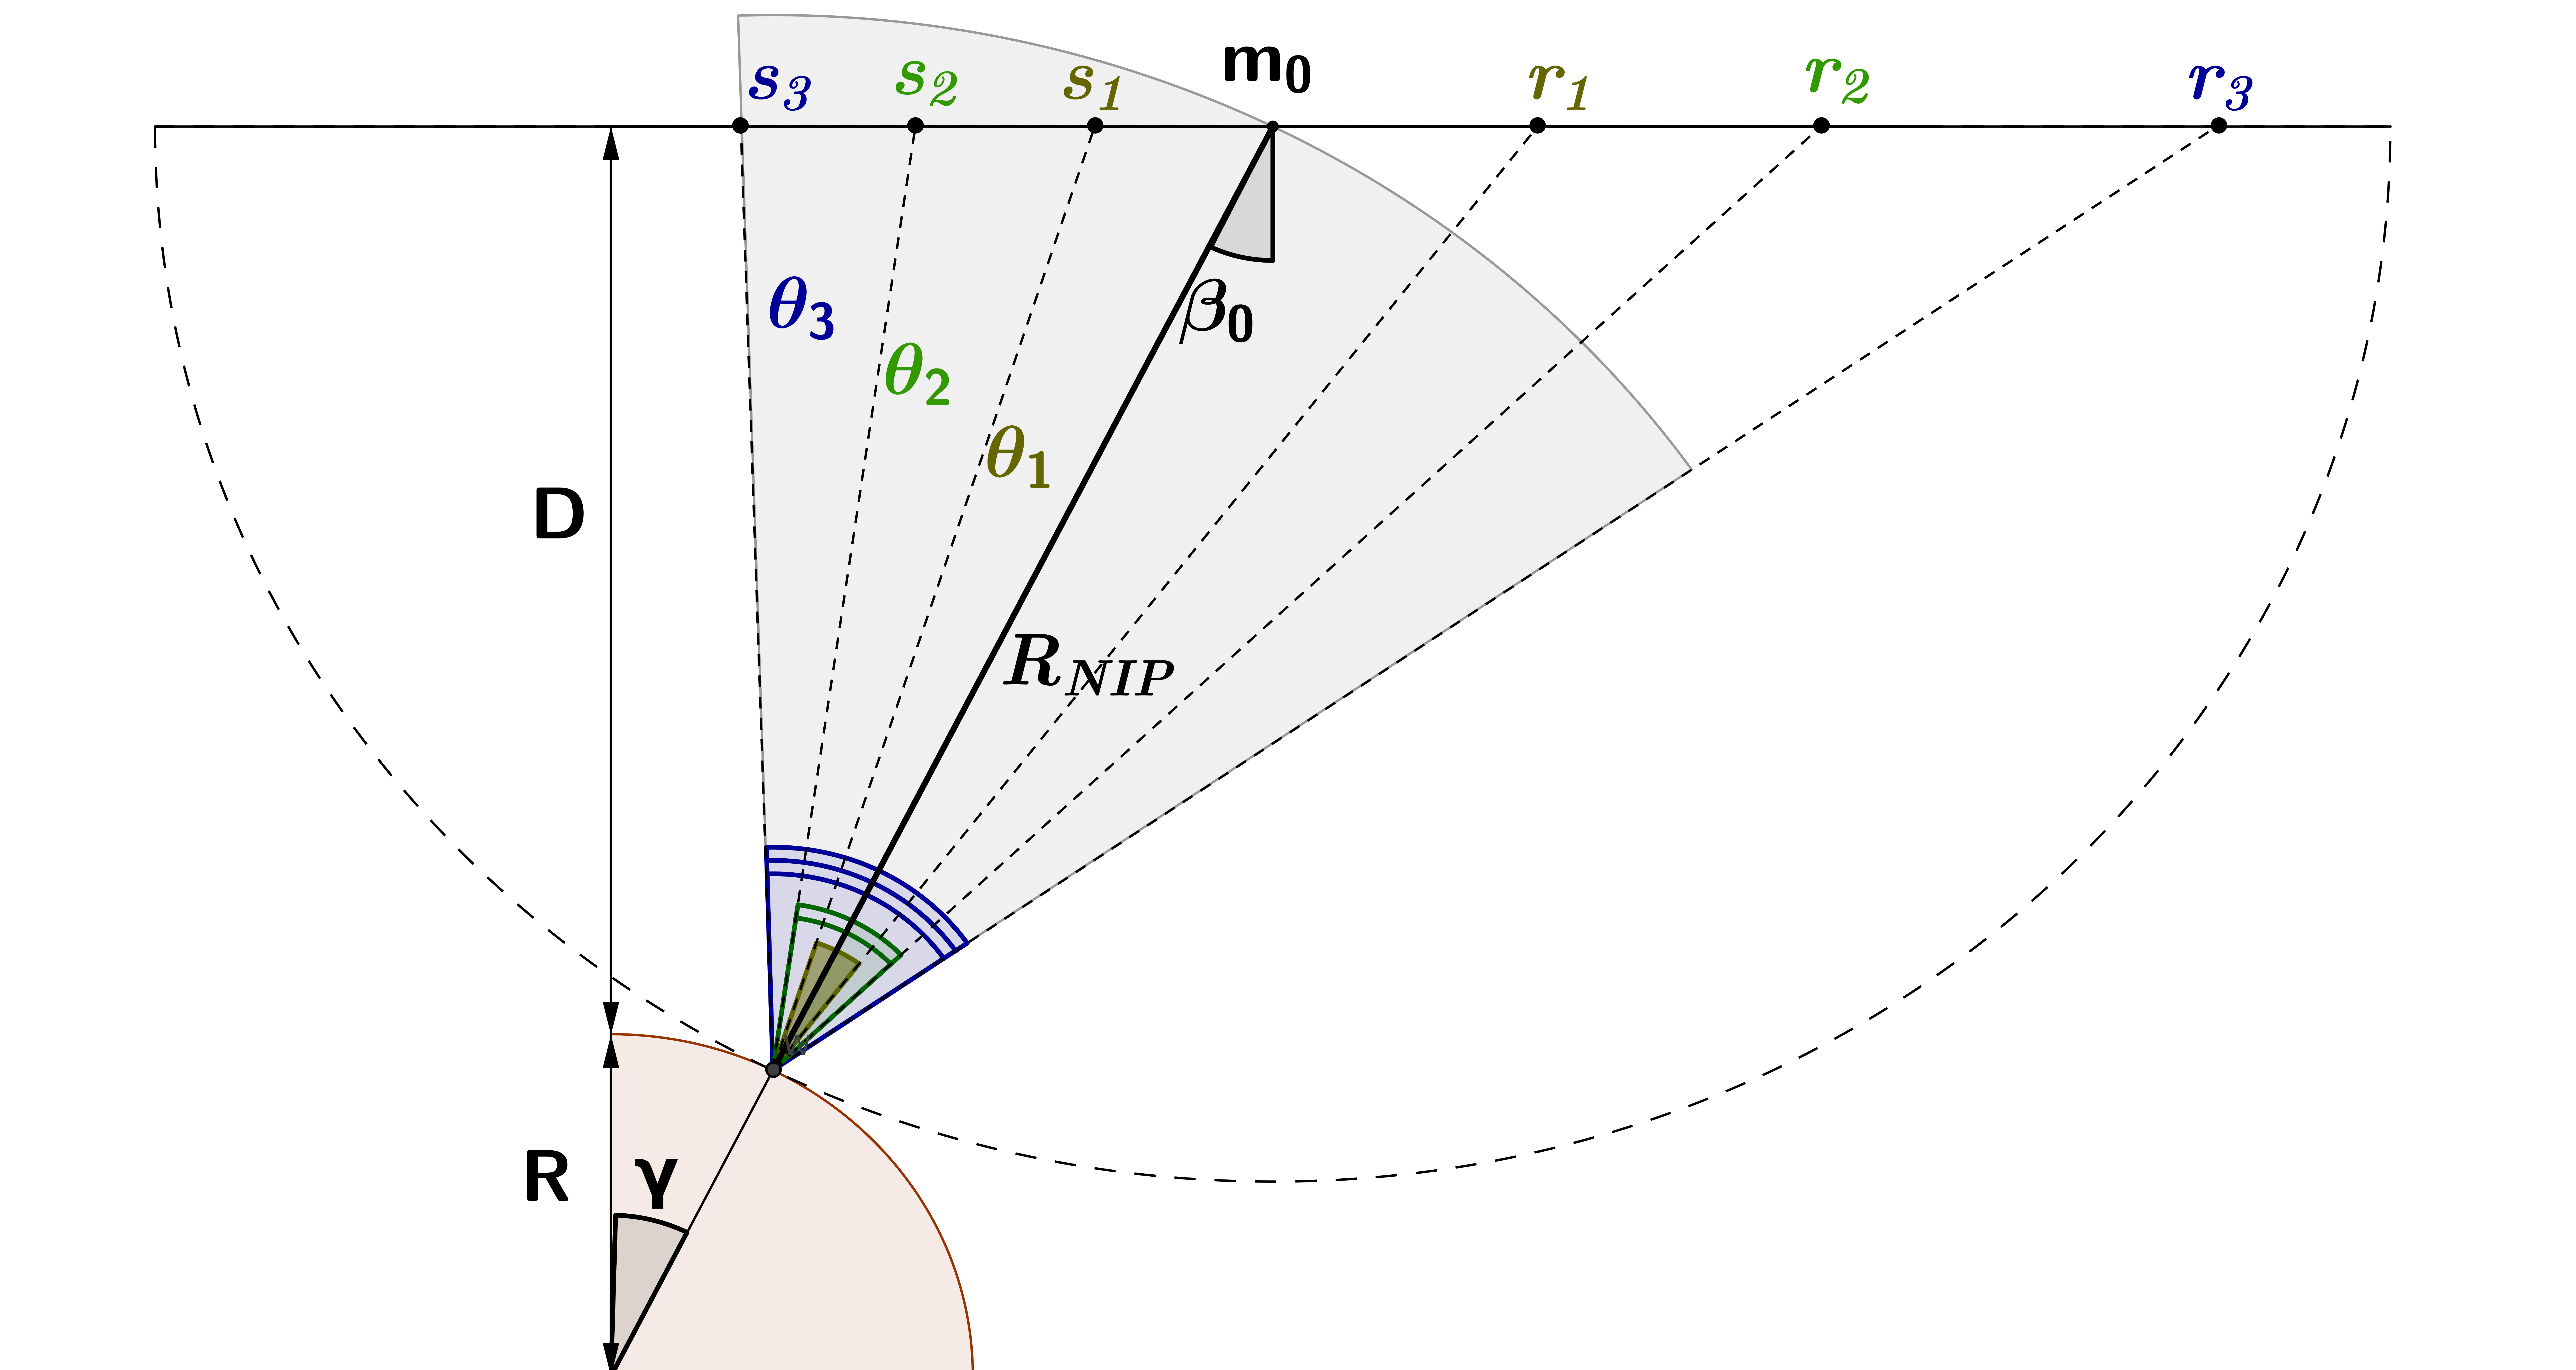
\includegraphics[scale=0.4]{images/cre.png}
\vspace{-0.3cm}
\end{center}
\begin{center}
 Fonte: Do Autor.
\end{center}
\label{fig:4.1}
\end{figure}


\begin{figure}[htb]
\caption{Representação esquemática das coordenadas do ERC sobre o modelo do refletor circular da Figura \ref{fig:4.1}:
Modificamos a posição do PMC central $m_0$ variando o ângulo $\gamma$ no modelo do refletor circular.
Ao variarmos o ângulo $\theta$, mantendo $\gamma$ constante, obtemos os pares $s_i$-$r_i$ (fonte-receptor)
dentro da família
ERC, as posições $h$ (meio afastamento) e $m$ (PMC) são obtidas para cada par fonte-receptor.
Cada curva colorida representa uma posição
diferente de $m_0$, um valor diferente de $R_{NIP}$ e $\beta_0$, e uma família ERC diferente.}
\begin{center}
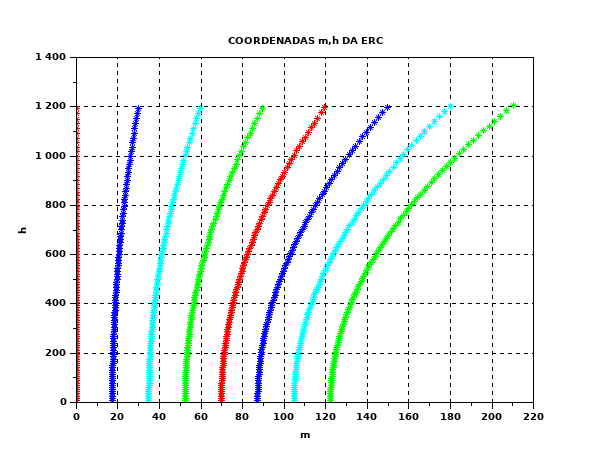
\includegraphics[scale=0.5]{images/coordenadas_CRE.png}
\vspace{-0.3cm}
\end{center}
\begin{center}
 Fonte: Do Autor.
\end{center}
\label{fig:4.2}
\end{figure}





O parâmetro de assimetria desenpenha um papel importante na seleção de pares fonte-receptor para os quais
o correspondente raio de reflexão refletem no mesmo ponto \cite{tygel}.




 %CRE
%\chapter{RESULTADOS PRELIMINARES (Pt. 2)}
\chapter{EXPERIMENTO NUMÉRICO SRC}
\label{cap5}

Realizamos um experimento numérico para testar a  acurácia das aproximações do SRC e a robustez da otimização
global utilizando o algoritmo VFSA: Os parâmetros do SRC que produzem o melhor
ajuste da aproximação do SRC escolhida aos dados modelados a partir das equações do modelo do refletor circular
serão obtidos a partir da inversão utilizando o VFSA.

O VFSA simula o resfriamento lento de cristais a partir de uma dada temperatura inicial arbitrária 
$T_0$, esta temperatura
decai a cada passo, enquanto os valores dos parâmetros $R_N$, $R_NIP$ e $\beta_0$ convergem para o melhor ajuste possível. 
Há ainda um fator de amortecimento $C_0$ para ajustar o intervalos dos passos ao problema, a
escolha de $C_0$ e $T_0$ é arbitrária.
Realizamos vários
testes e descobrimos por tentativa e erro que os valores de $C_0$ e $T_0$ que melhor se ajustam ao experimento
proposto são $C_0=0.5$ e $T_0=10$.
Contamos cada convergência dos parâmetros $R_N$, $R_NIP$ e $\beta_0$ como uma iteração,
realizando ao todo  10 iterações cada uma com 25000 passos de atualização de temperatura.
O parâmetro otimizado é a média do valor do parâmetro obtidos em cada iteração, para evitar
ruído aleatório na obtenção dos parâmetros.
O experimento numérico é descrito a seguir:

\begin{enumerate}
 \item Obtivemos a superfície de tempo de trânsito SRC modelada com as Equações \ref{eq:7.1}-\ref{eq:7.3}
 para o modelo do refletor circular da Figura \ref{fig:7.1}, com os parâmetros definidos: $D=1000m$, $R=1000m$, 
 $v_0=1500m$. Para o PMC central $m_0$ escolhido arbitrariamente...
 
 \item Utilizamos o algoritmo VFSA para encontrar os parâmetros o algoritmo gera um valor dos parâmetros $R_N$, $R_NIP$ e $\beta_0$
 e produz a superfície SRC aproximada utilizando uma aproximação do SRC escolhida, compara a aproximação do SRC com
 a superfície SRC modelada a partir da coerência (Semblance). O melhor ajuste será produzido ao atingir o valor máximo da
 coerência entre a superfície aproximada do SRC e a superfície modelada.
 
 \item Calculamos o erro relativo entre os parâmetros obtidos através da otimização com o VFSA
 e os parâmetros do modelo, obtidos a partir
 das Equações \ref{eq:7.4}-\ref{eq:7.7}. 
 
 \item Apresentamos o erro relativo absoluto entre a superfície otimizada e
 a superfície modelada. As regiões de melhor ajuste estão em azul, e as regiões de pior ajuste estão em vermelho.

\end{enumerate}




500<rn<3000
500<rnip<3000
-pi<beta0<pi
 %CRS JC/PEDRO CHIRA
 \chapter{EXPEIMENTO NUMÉRICO ERC}
\label{cap6}

Realizamos um experimento numérico para testar a  acurácia das aproximações do SRC com os parâmetros do SRC obtidos a partir
do VFSA.

1. Obtivemos a superfície de tempo de trânsito SRC modelada com a Equação \textbf{TAL} para o modelo do refletor circular,
os parâmetros da geometria do modelo estão na tabela a seguir:

\textbf{TABELA}

Utilizamos o algoritmo VFSA para obter os parâmetros do SRC que melhor ajustam a aproximação do SRC escolhida a superfície de
tempo de trânsito modelada, estes são os parâmetros otimizados

Comparamos o erro relativo absoluto entre a superfície otimizada e a superfície modelada
As regiões de melhor ajuste estão em azul, e as regiões de pior ajuste estão em vermelho, apresentamos também uma tabela
com os parâmetros SRC otimizados versus modelados para comparação. %ESTUDO REFLETOR CIRCULAR
 \chapter{OBJETIVO}
\label{objetivo}


 %CONCLUSÃO
% \chapter{CONCLUSÃO}
\label{cap8}

As equações do tempo de trânsito utilizando aproximantes de Padé 
surgem como alternativa para aproximar o tempo de trânsito em grandes afastamentos
são mais acuradas do que a aproximação hiperbólica do tempo de
trânsito (sobretempo normal). Estas aproximações dependem apenas de 3 parâmetros,  $v$,  $t_0$ e o parâmetro $A$,
obtido
através da expansão em série de Taylor de quarta ordem do tempo de trânsito ao longo do raio normal.

As aproximações do SRC utilizando aproximantes de Padé, são mais acuradas que a aproximação hiperbólica do SRC. 
As aproximações
não hiperbólicas do SRC: SRC Padé, SRC não hiperbólico e SRC quarta ordem, estendem a região de convergência da aproximação
hiperbólica do SRC para maiores distâncias entre os pontos médios e meio afastamentos, surgindo como alternativa 
para a realização do empilhamento através de superfícies SRC não hiperbólicas que estendem a região de empilhamento,
aumentando a cobertura e razão sinal/ruído.

A aproximação \textit{quadrática} do SRC quarta ordem produziu o melhor ajuste na inversão dos parâmetros do SRC
através da otimização por mínimos quadrados. 
Isso sugere que, apesar do método de inversão utilizado
tornar complicada a utilização das aproximações SRC Padé por causa da dificuldade
em calcular as derivadas parciais
necessárias, utilizando outro método de inversão dos parâmetro do SRC que não necessite dessas
derivadas,
a região de convergência obtida tenderia a aumentar através da introdução das aproximações SRC Padé.


Como sugestão para pesquisas futuras propomos a realização das etapas de empilhamento, tanto para a configuração 
ponto médio comum quanto SRC, sobre as curvas e superfícies produzidas através das aproximações de Padé. 
Enfatizando que as aberturas no domínio do afastamento e dos pontos médios irá influênciar na diferença
de acurácia nas seções empilhadas. Uma vez, que a melhora na acurácia das aproximações não hiperbólicas em
relação as aproximações sobretempo normal e SRC hiperbólico, surge
para grandes afastamentos e distâncias entre os pontos médios.
O parâmetro $A$ pode
ser obtido através de \textit{Semblance}, para encontrar o parâmetro
que melhor ajusta a curva aos dados para grandes afastamentos, a velocidade
utilizada na aproximação será a $v_{RMS}$. No caso SRC, uma vez obtidos os parâmetros $R_N$,
$R_{NIP}$ e $\beta$ bastará substituí-los nas aproximações SRC Padé e realizar 
o empilhamento sobre as superfícies SRC aproximadas.


%% ---
\bookmarksetup{startatroot}% 
%% ---
%% ----------------------------------------------------------
%% Referências bibliográficas
%% ----------------------------------------------------------
\bibliography{mybib2}
%
%% ----------------------------------------------------------
%% Glossário
%% ----------------------------------------------------------
%%
%% Consulte o manual da classe abntex2 para orientações sobre o glossário.
%%
%%\glossary
%
%% ----------------------------------------------------------
%% Apêndices
%% ----------------------------------------------------------
%
%% ---
%% Inicia os apêndices
%% ---
%\begin{apendicesenv}
%
%% Imprime uma página indicando o início dos apêndices
%\partapendices
%\newpage\null\thispagestyle{empty}
%\begin{center}
%\vspace{10cm}
%{\large\textbf{APÊNDICES}}
%\end{center}
%\newpage

%% ----------------------------------------------------------
%\chapter{Quisque libero justo}
%% ----------------------------------------------------------
% \input{apendiceA}
% \input{apendiceB}
% \input{apendiceC}
% \input{apendiceD}
% \input{MT}
%
%\end{apendicesenv}
%% ---
%
%
%% ----------------------------------------------------------
%% Anexos
%% ----------------------------------------------------------
%
%% ---
%% Inicia os anexos
%% ---
%\begin{anexosenv}
%
%% Imprime uma página indicando o início dos anexos
%\partanexos
%
%% ---
%\include{AnexoA}


%% ---
%\lipsum[30]
%
%% ---
%\chapter{Cras non urna sed feugiat cum sociis natoque penatibus et magnis dis
%parturient montes nascetur ridiculus mus}
%% ---
%
%\lipsum[31]
%
%% ---
%\chapter{Fusce facilisis lacinia dui}
%% ---
%
%\lipsum[32]
%
%\end{anexosenv}

%---------------------------------------------------------------------
% INDICE REMISSIVO
%---------------------------------------------------------------------

\cleardoublepage
\phantomsection 
\printindex

\end{document}
